







\documentclass[3p,twocolumn,authoryear,10pt]{elsarticle}
\usepackage{graphicx}
\usepackage{amsmath, amsthm, amssymb}
%\usepackage{outline}
\usepackage{colortbl}
\usepackage[no lists,figuresfirst]{endfloat}
\usepackage{rotating}
\usepackage{multirow}
\usepackage{setspace}
\usepackage{arydshln}
 
\usepackage{color,soul}

\journal{Journal of Experimental Psychology: General}

\begin{document}

\begin{frontmatter}


\title{Using Mechanical Turk for Experimental Psychology Research: Replicating a classic finding online.\tnoteref{t1}}


\author[nyu]{John McDonnell\corref{cor1}}
\ead{John McDonnell <john.mcdonnell@nyu.edu>}

\author[nyu]{Devin Domingo}
\ead{Devin Domingo <devdomingo@gmail.com>}

\author[nyu]{Todd M. Gureckis}
\ead{todd.gureckis@nyu.edu}

\cortext[cor1]{Corresponding author}

\address[nyu]{New York University}

\tnotetext[t1]{The authors thank Bob Rehder, Greg Murphy, Nathaniel Daw, Larry Maloney, Eric Taylor, and the NYU ConCats group 
for helpful discussions in the development of this work. Correspondence concerning this research should be addressed to Doug Markant, Department of Psychology, New York University, 6 Washington Place, New York, NY 10003. Email: doug.markant@nyu.edu.
}

\begin{abstract}
Is Internet-based data collection the future of cognitive science research? We used Amazon's Mechanical Turk (AMT) to replicate a classic result in cognitive psychology which has primarily been established under traditional laboratory conditions (Shepard, Hovland, Jenkins, 1961).  In this post, we describe the various lengths we went to in order to get useful data from AMT and what we learned in the process.  Overall, our results highlight the potential for using AMT in experimental research, but also raise a number of concerns and challenges. We invite comments, discussion, and shared experience below!
\end{abstract}

\end{frontmatter}

\section{Introduction}


One challenging aspect of experimental psychology research is the constant struggle for data. Typically, we depend on university undergraduates who participate in studies in exchange for experience, course credit, or money. Research progress depends on the ebb and flow of the semester. As a result, it can take weeks, months, or even years to conduct a large behavioral study. This issue is even more salient for researchers at smaller universities.


One solution to this problem could be to recruit participants outside of the traditional undergraduate psychology "pool." In fact, there are a number of convincing scientific arguments that over-dependence on undergraduate student populations for psychological research may be flawed (Henrich, Heine, and Norenzayan, 2010). One appealing idea is to collect data over the Internet. In theory, online experimentation would allow researchers to collect data internationally, enable access to a very large number of people who may be interested in participating in research studies, and can be fairly automated. However, the main obstacle to conducting Internet-based research is finding people who are willing to participate and compensating them. Sure, you can post a link on your webpage, but few people are likely to find it.

\subsection{Enter Mechanical Turk}

Recently, our lab (like a number of others) has explored the possibility of using Amazon's Mechanical Turk(AMT) for behavioral data collection. AMT is a crowdsourcing or "artificial-artificial-intelligence" platform, in which people submit simple computer-based "jobs" to human workers online (see Box 2).

While Internet-based methods for collecting data have been around for a while, AMT is a potentially useful system for researchers since it handles both recruitment and payment in a fairly automatic way. There are a large number of people who use AMT making it a great way to advertise and distribute studies (some websites report over 100,000 users).

Recently, there have been a number of excellent summaries and workshops about using AMT for research. Most notably, Winter Mason of the Stevens Institute of Technology has a Behavior Research Methods paper, which summarizes how to use the system and what it does (see also this excellent blog post and the references below).

Rather than focus onhow to use AMT, this post focuses on the reliability of the data for experimental research in cognitive psychology. Along those lines, we had a couple of questions going into this project:
	First, could we replicate classic findings in cognitive psychology concerning learning and memory processes with fidelity similar to that collected in the lab?
	Second, what unexpected issues come up in conducting learning, memory, and reasoning studies online?
	Third, how reliable is data on AMT as a function of the payment amount?

In this sense, our analysis is similar to a couple of recent papers (e.g., Paolacci, Chandler, and Ipeirotis, 2010 and Buhrmester, Kwang, and Gosling, 2011). However, these previous reports focus on survey data, the test-retest reliability of AMT, or on simple one-shot decision making tasks. In contrast, we were interested in using AMT to replicate and extend classic findings in experimental cognitive psychology which were originally established in the lab. Our emphasis was not just on qualitative replication, but in getting quantitatively accurate data in a study that has been frequently replicated in the lab.  In addition, we wanted to explore what happens in Internet-based experiments which unfold over many trials, require learning, sustained attention, and which may require between 20-60 minutes to complete.

Our initial experiments provide answers to many of these questions, and we felt our results might interest people thinking of using AMT for their own experiments.


\subsection{Taking experiments online}

In terms of taking cognitive experiments online, there are a number of unique challenges compared to simple ratings tasks or surveys.

First, such experiments usually take extended time (on the order of 1 hour) and uninterrupted concentration which may or may not be amenable to the AMT, which typically emphasizes short, one-shot human judgment tasks or surveys. In our initial test, we have tried to keep our tasks shorter than usual (roughly 15-30 minutes).

Second, compared to a simple HTML survey, the visual display in many cognitive experiments is typically dynamic (things may move around, there may be animations, people may respond by manipulating objects on the screen with the mouse, etc...). This raises a couple issues about how to control the screen display to ensure that people using many different types of computers (netbooks, iPads, regular desktops) view roughly the same thing. In addition, ensuring the experiment can even run without hassle in the Worker's browser can be a technical challenge. For example, what happens when the Internet connection intermittently fails in the middle of your experiment or the browser window is closed?

After initial testing and research, we decided that there is no general solution to these issues and it is up to the individual to balance ease-of-programming with the ability to support many diverse computer systems (this will be discussed more in an upcoming post). For example, we ran into difficulty in providing support for Internet Explorer in our task. It might have taken an extra two or three weeks to figure out all the idiosyncrasies of the various rendering engines and Javascript implementations in every browser. However, it turns out that most users on AMT do not use Internet Explorer so this decision has (hopefully) modest consequences.

Ultimately, there are many options available for designing web-based experiments that run in a browser and if you are savvy enough you can probably do 80\% of what Matlab's Psychophysics toolbox does. We found it fairly simple to design a dynamic display with Javascript that did not require extensive browser reloading between trials: All stimuli load at the beginning of the experiment and run as a web-app in the user's browser sending us updated data at the end of each block. Ultimately, our philosophy was to make our programming job easy (and bug free!) and to try to cover the majority of computer systems.





\section{Experiment 1: A replication of Shepard, Hovland, and Jenking (1961)}

The experiment examines self-directed learning in the context of a relatively simple and well-studied perceptual learning task using multidimensional, continuous-valued stimuli~\citep{Ashby:1998p8468,Ashby:2002p13331}.  The principal manipulation is to compare categorization performance in a standard, ``passive" learning condition to an alternative, ``self-directed" condition in which learners could actively sample category members they wanted to learn about on each trial.   

In the task, participants learned to classify perceptual stimuli into one of two groups.  Two types of abstract category structures were used: (1) a \textit{rule-based} (RB) structure, in which the optimal classification rule is a criterion along a single dimension, and (2) an \textit{information-integration} (II) structure, in which the decision rule is a linear function of two dimensions (see Figure~\ref{design.fig}A). We anticipated that participants' self-directed learning ability would vary between the RB and II learning tasks. Previous research has suggested that these two category structures may be learned in fundamentally different ways~\citep{Ashby:1998p8468}. In particular, RB categories are thought to be learned by reasoning about verbal or explicit hypotheses, while the structure of II categories precludes a simple verbal description and is instead thought to be learned via implicit or procedural learning. Critically, it is often assumed that learners initially prefer to try out simple, uni-dimensional rules and only abandon that strategy following extensive trial-and-error training (i.e., in the II task). We hypothesized that self-directed learning may be most effective when participants are considering simple rules, and would thus lead to an advantage in the RB case because the category structure aligns with the default strategy people bring to the task~\citep{Ashby:1999ig,Kruschke:1993ty}. 

 \begin{figure}[t]
\centerline{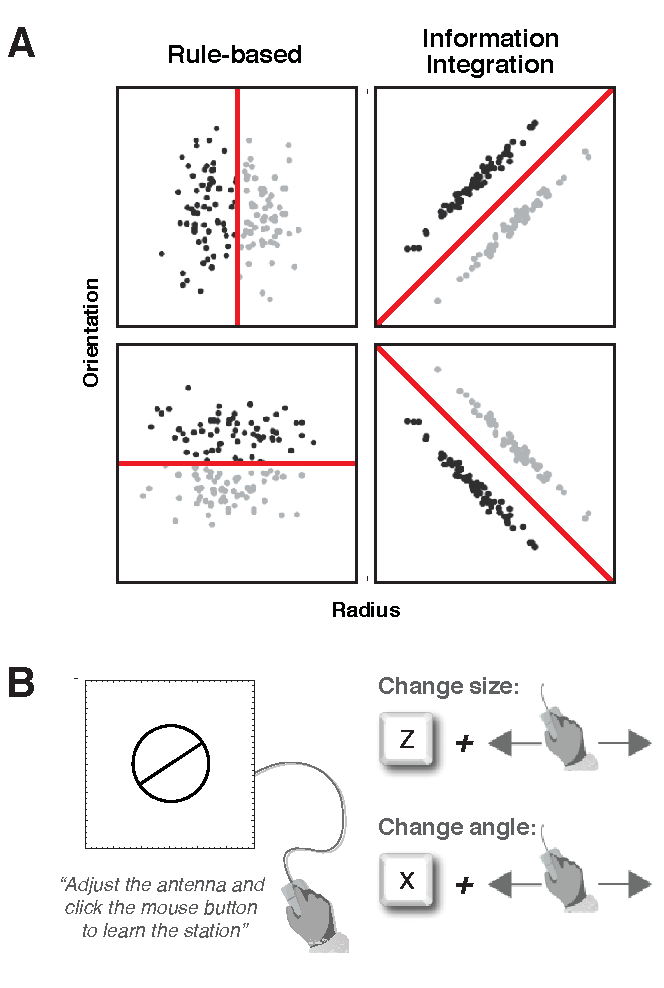
\includegraphics[width=2.9in]{figures/taskdesign.pdf}}
\caption{\textbf{A:} Examples of the rule-based (RB) and information integration (II) category distributions.  The space of stimuli is defined by two dimensions (orientation and radius, see panel B for an example stimulus).  Each point in the space corresponds to a particular stimulus with a given value along each dimension.  The clouds of points illustrate an example distribution of training stimuli shown to participants in the passive-normal condition, while the solid line is the optimal decision boundary. Participants in the self-directed learning condition received feedback consistent with this optimal boundary even though their training distribution differed from the training distribution plotted here.  \textbf{B:} A depiction of a stimulus (left) and the interface used in the self-directed learning condition.}
\label{design.fig}
\end{figure}


In addition to the two category structures, participants in the experiment were further divided into four training conditions. In the \textit{self-directed} (S) condition, participants ``designed" stimuli in order to reveal their category membership. In the \textit{passive-normal} (P) condition, participants observed training stimuli that were randomly generated from two bivariate normal distributions (i.e., a standard training procedure for these types of tasks).
  In the final two training conditions, participants were ``yoked" to the sequence of observations made by participants in the self-directed condition, but learned through passive observation. In the \textit{Na\"ive passive-yoked} (Y1) condition, participants were not given any information about the source of their training data (i.e., they were in the same informational state as the passive-normal participants). In the \textit{Aware passive-yoked} (Y2) condition, participants were told that their data had been selected by a previous participant  in the task with the same learning objective but who had been learning in a self-directed way.



%There are three key aspects of the design worth highlighting. First, in binary classification tasks, a highly effective information sampling strategy is simply to make queries close to the current estimate of the category boundary (where uncertainty is highest), a region referred to as the ``margin." 


%Moreover, since successful learning in the II task may be contingent on abandoning rule-based strategies in favor of procedural learning, self-directed learning might even lead to a learning \textit{impairment} for the II structure by encouraging perseveration in the search for a sub-optimal rule.


Our goals in the design were three-fold. First, we were interested in whether self-directed learners 
could adaptively structure their own learning experience in order to acquire a new concept more
quickly than through passive, observational training. The comparison of self-directed 
learners with the passive-normal group allowed us evaluate this advantage above and beyond 
the typical training procedure in such tasks.

Second, we were interested in how the effectiveness of self-directed sampling might interact with
differences in abstract category structure. While a number of recent studies have explored how learners make information sampling decisions to support their own learning~\citep{Nelson:2005ph,Castro:2008p12850,Kruschke:2008ph,Gureckis:2009p13894,Steyvers:2003p5901}, there has not yet been a systematic evaluation of how this ability might depend on the form of category being learned.

Finally, the inclusion of the passive-yoked training groups allowed us to separately evaluate the impact of 
selecting samples from the statistical information contained in those samples (since the distribution of training 
data is identical for both groups). Previous research suggests that active or intervention-driven learning may 
lead to advantages over yoked learning~\citep{Lagnado:2004p13374,sobel2006importance,Steyvers:2003p5901}, but it is unclear whether these results would generalize to both of the abstract category structures tested here. In addition, a factor that has not been examined in previous work is whether awareness of the yoking procedure is sufficient to overcome this disadvantage, which we test with our comparison between ``na\"ive" and ``aware" passive-yoked groups.

%Second, we were interested in how the effectiveness of self-directed sampling might interact with previously studied differences in category structures. While a number of recent studies have explored how learners make information sampling decisions to support their own learning~\citep{Nelson:2005ph,Castro:2008p12850,Kruschke:2008ph,Gureckis:2009p13894,Steyvers:2003p5901}, there has not yet been a systematic evaluation of how this ability might depend on the form of category being learned.

%Additionally, it is unclear how the engagement of additional metacognitive processes during active learning would affect performance during the II task. 

% At various intervals during the experiment, participants were given test trials which
%assessed their classification accuracy over the entire stimulus space.  Our primary dependent
%measure was the rate at which learners acquired the categories in either condition, as well
%as the distribution of samples that participants chose in the active learning condition.

%There are several key aspects of our design and hypotheses worth highlighting.  In particular,
%in our experiment, we compare conditions of active learning  to standard passive training 
%(akin to the learning-by-doing versus learning-by-observing distinction described above).  Critically, 
%in each situation we included a third, yoked condition where learners were given the 
%samples chosen by an active learner under passive learning conditions.  This allows us to 
%separately quantify the impact of actually selecting samples from the statistical information 
%contained in those samples (since the distribution of examples viewed in the passive and active
%condition were quite different).  



%\begin{figure}[t]
%\centerline{\includegraphics[width=3.8in]{figures/activepassiveinterface.pdf}}
%\caption{{An example of the stimuli (left) and interface used in the active-learning condition.  Participants used their mouse to ``design" stimuli.  Clicking the mouse would reveal the category label associated with the item.}}
%\label{interface.fig}
%\end{figure}


%Our selection of the RB and II category structures also offers a number of interesting
%contrasts.  Previous research using these two types of category structures has 
%suggested that they are learned in fundamentally different ways~\citep{Ashby:1998oa,Ashby:2001ul}.
%In particular, RB categories are often assumed to be learned using a set of verbal
%rules and explicit hypotheses.  In contrast, the structure of II categories precludes a simple
%verbal description and are instead assumed to be learned via implicit, procedural learning.
%To the degree that participants are able to leverage their current uncertainty
%about the category to construct informative samples at all, this ability may be more effective
%in the RB condition where the category distinction can be better articulated.  Indeed, active
%learning may engage extra meta-cognitive and reasoning processes which actually impair the 
%learning of information-integration categories.  

%Thus, the relative 
%advantages of active/passive may interact with the 
%actual structure of the category.  
%Finally, the alignment of our paradigm with previous research
%means a subset of our condition are approximate replications 
%of  previously published findings~\citep{Ashby:2002p13331} and thus provide a more rigorously specified baseline
%against which to compared passive learning.   
%  Given 
%that active learning likely involves the engagement of meta-cognitive processes about what is or isn't 
%currently known about the category, it is likely that the success of active learning may depend on the 
%structure of the
%category.

%In addition to our empirical results, we also propose a model-based explanation for the pattern of results we observe across conditions. Our modeling approach builds upon previous theories of the computational processes that underly human categorization, captured by the ``rational model" formalism first proposed by~\citep{Anderson:1991hd} and extended by~\citep{Sanborn:2006kx}.  In our extension to these models we consider how uncertainty about the true category can be converted into a information sampling strategy.  Comparing the predicted sampling strategy of the model and human participants provides
%insight into the strategies that people use to collect information when learning. Second, using the model we propose an explanation for why active learners might out-perform passive learners, even given the exact same set of observations.

%  Quantitative 
%models are proposed that analyze the evolution and efficiency of this search behavior relative 
%to a number of normative frameworks.

%Finally, in the paper we proposed a model-based explanation for our pattern of our results
%in terms of a popular model of human category learning based on Bayesian learning principals.
%Our approach ry
%inference is to infer the underlying cluster structure of a set of stimuli (see also~\citep{Love-2004bp}).   
%We begin be reviewing previous work on learning-by-doing from a cognitive perspective, then
%describe our experiment.  We conclude with a set of simulations which help explain the
%pattern of results we find that are grounded in contemporary theories of human concept learning.

%\subsection{Is active learning better than passive learning?}


%Despite this, little work has directly explored
%if people can themselves adopt effective exemplar sequencing as would be implied by theories of ``active learning."  
%Ultimately, there remains great opportunity to explore the terrain between active and 
%entirely passive learning.  To quote Gigerenzer,

%
%Some active learning background. 

%
%\subsection{The Present Experiment}

%
%Despite its potential impact on human learning, there has traditionally been little emphasis on information selection in category learning domains. For example, many studies have examined learning in perceptual categorization tasks, in which the goal is to partition previous observations according to an unknown category boundary~\citep{ashby1992complex,Ashby:2002jt}. These studies have shown that the form of the category boundary influences the speed and flexibility of learning. In particular, if the category boundary is defined as a criterion on a single dimension (i.e., ``rule-based," or RB), people acquire the category distinction quickly and are insensitive to the type of feedback being used (i.e., observational or feedback error)~\citep{Ashby:2002p13331}. In contrast, when the category boundary is a function of two dimensions (i.e., ``information-integration"), learning proceeds more slowly and is influenced by variations in feedback and timing, among other task variables. A prominent theory of this type of category learning suggests that these two classes of problems engage different learning systems. 

%While detailed models of participants' performance in these tasks have been described, they make no assumptions regarding the learner's trial-by-trial uncertainty during the task. What are some other proposals for this? 

%Evidence suggesting that RB and II categories are learned by separate systems may have implications for whether people are able to leverage their uncertainty to select useful information during learning. 

%Eventually, as all the particles 
%converge on a single solution the disagreement over the labeling of different items will 
%drop, at which point the learner should become indifferent to alternative samples.


%
%\begin{equation}
%\label{prior}
%P(z_i=k|\textbf{z}_{i-1}) = 
%\begin{cases} \frac{cM_k}{(1-c)+c(i-1)} \text{if $M_k>0$ (i.e., k is old)} \\
%		      \frac{1-c}{(1-c)+c(i-1)} \text{if $M_k=0$ (i.e., k is new)} 
%\end{cases}
%\end{equation}

%\begin{equation}
%\label{posterior}
%P(z_i=k|\textbf{z}_{i-1},\textbf{F}_i) 
%\end{equation}

\subsection{Methods}
 
\subsubsection{Participants}
Two hundred forty undergraduates at New York University participated in the study. The experiment was run on standard Macintosh computers in a single 40 min session. Each participant was assigned to either the rule-based (RB) or information-integration (II) task, and to one of four training conditions: self-directed (S), passive-normal (P), na\"ive passive-yoked (Y1), or aware passive-yoked (Y2).

\subsubsection{Stimuli and Materials}
Stimuli were defined by a two-dimensional continuous-valued feature space, where one dimension corresponded to the size (radius) of a circle and the second dimension corresponded to the angle of a central diameter (see example in Figure~\ref{design.fig}B). Stimuli of this type have been used in many studies of perceptual classification \citep[e.g.,][]{Garner:1970fk,Shepard:1964xf,Nosofsky:1989gu} and previous work has established that these two dimensions are, for most subjects, separable and independent~\citep{Nosofsky:1989gu}.
Stimuli could be assigned a value on each dimension within the range [1,600]. These values were converted for display such that there was a limited range of possible orientations and sizes. The orientation of the stimulus could vary over 150 degrees, ensuring that a full rotation of the stimulus was not possible. The minimum radius and orientation was randomized so that the optimal decision boundary corresponded to a unique location in perceptual space for each participant. 

One-hundred and twenty-eight training stimuli were created for the passive-normal training condition using random samples from two bivariate Gaussian distributions (see Figure~\ref{design.fig}A) with mean and covariance parameters slightly modified from~\citep{Ashby:2002p13331}. For classification trials, a uniform grid of 256 unique test items was generated over the feature space for use in all conditions. For each test block, eight stimuli were randomly chosen (without replacement) from each quadrant of the stimulus space (to avoid random biases in the test distribution), for a total of 32 items in each block. The order of individual test items within each block and the order of the eight test blocks were both randomized for each participant.



%In order to avoid chance clustering of test items (i.e., a unbalanced number of item coming from the same region of the stimulus space), quadruples of stimuli (containing a single test item from each quadrant of the space) were sampled from the uniform grid without replacement. Four random quadruples were chosen for each test block, and for each participant the presentation order of the quadruples was then randomized.


\subsection{Procedure}
Participants were told that the stimuli in the experiment were ``loop antennas" for televisions, and that each antenna received one of two channels (CH1 or CH2). They were told that the channel received by any antenna depended in some way on the two dimensions described above, and the participant's goal was to learn the difference between the two types of items. Participants were instructed that the antennas were sometimes ``noisy" and could pick up the wrong channel and that it would be beneficial to integrate over a number of trials during learning. In the experiment, however, the feedback associated with each item was deterministic. The experiment consisted of 8 blocks, with each block divided into a set of 16 training trials followed by 32 test trials. \\



\begin{table}[t] \caption{\small Category distribution parameters used in the experiment for the passive-normal (P) condition. Within each task (RB/II), participants were randomly assigned to one of the two category structures shown in Figure~\ref{design.fig}A.} % title of Table 
\centering      % used for centering table 
\begin{tabular}{ l c c c c c c }  % centered columns (4 columns) 
& \textbf{\small $\mu_x$} & \textbf{\small $\mu_y$} & \textbf{\small $\sigma_x^2$} & $\small{\sigma_y^2}$ & \textbf{\small $cov_{xy}$}\\ [0.1ex] % inserts table 
%heading 
\hline                    % inserts single horizontal line 
\multicolumn{3}{l}{\textbf{\small Rule-Based (RB)}}  &  &  & \\ [0.5ex] % inserts table 
  \multicolumn{1}{c}{ \textit{\small 1. Category A}} &   \small{220} &  \small{300} &  \small{2000} &  \small{9000} &  \small{0} \\ [0ex] % inserts table 
   \multicolumn{1}{c}{\textit{\small \hspace{.1in} Category B}} &   \small{380} &  \small{300} &  \small{2000} &  \small{9000} &  \small{0} \\ [1.5ex] % inserts table 

  \multicolumn{1}{c}{\textit{\small 2. Category A}} &   \small{300} &  \small{220} &  \small{9000} &  \small{2000} &  \small{0} \\ [0ex] % inserts table 
   \multicolumn{1}{c}{\textit{\small \hspace{.1in} Category B}} &   \small{300} &  \small{380} &  \small{9000} &  \small{2000} &  \small{0} \\ [1.5ex] % inserts table 

\hline
\multicolumn{3}{l}{\textbf{\small Information-Integration (II)}}  &  &  & \\ [0.5ex] % inserts table 
   \multicolumn{1}{c}{\textit{\small 1. Category A}} &    \small{250} &  \small{350} &  \small{4538} &  \small{4538} &  \small{4463} \\ [0ex] % inserts table 
   \multicolumn{1}{c}{\textit{\small \hspace{.1in} Category B}} &    \small{350} &  \small{250} &  \small{4538} &  \small{4538} &  \small{4463} \\ [0.5ex] % inserts table 

   \multicolumn{1}{c}{\textit{\small 2. Category A}} &    \small{250} &  \small{250} &  \small{4538} &  \small{4538} &  \small{-4463} \\ [0ex] % inserts table 
   \multicolumn{1}{c}{\textit{\small \hspace{.1in} Category B}} &    \small{350} &  \small{350} &  \small{4538} &  \small{4538} &  \small{-4463} \\ [0.5ex] % inserts table 
\hline
\end{tabular} 
\label{catparams.tab}  % is used to refer this table in the text 
\end{table} 


\textit{Training phase -- All conditions}. The overall design of the training phase roughly matched the ``observational learning" procedure used by Ashby et al. (2002).  In that study, participants viewed a stimulus for a short, fixed duration followed by the corresponding category label of the stimulus for a fixed duration (the ``no response/after" condition).  Critically, participants were not asked to make an explicit prediction and corrective feedback was never provided.  The observational learning procedure is ideal for studying self-directed learning since we wanted to limit the conflicting demands of sampling informative items and sampling items which would result in ``correct" feedback under a supervised procedure.\\

\noindent
\textit{Training -- Self-directed Condition (S)}.  On each training trial the participant ``designed" a TV antenna and learned about its category membership. Each trial began with the presentation of a randomly generated stimulus in the center of the screen. The participant could then alter its size and orientation by moving the mouse from left to right while holding down either the `Z' or `X' key (see Figure~\ref{design.fig}B). The direction of motion and mapping of keys to features were randomized across participants. Only one dimension could be changed at a time, but participants could make any number of changes and use as much time as needed. When the stimulus was the desired size and orientation, participants pressed the mouse button to reveal the category label, which appeared above the stimulus and was visible for 1500ms. Querying the category label was not permitted until the participant had made a change to the initial stimulus. Trial duration was recorded starting with the initial presentation of the stimulus until the end of the trial. \\

\noindent
\textit{Training -- Passive-Normal Condition (P)}.  In the passive-normal condition, participants were unable to interact with the stimuli in any manner. Instead, in each trial they were presented with a stimulus generated from the category distributions described in Table~\ref{catparams.tab}. On each trial, a fixation cross was presented, followed by the stimulus (for 250ms), followed by the category label and stimulus together.  Out of concern that in this passive, observational condition participants might not pay attention during the learning phase (relative to the S participants who interacted with the display), the participant was required to press a key corresponding to the displayed category in order to end the trial.  The stimulus and label remained visible on the screen until the verification response was registered\footnote{In this design passive participants are not matched to self-directed participants in terms of perceptual-motor demands (e.g., precisely  adjusting the stimulus before observing the category label). However, pilot data suggested that attempting to equate this interaction (e.g., having passive learners adjust the stimulus to a pre-specified ``target") made learning much more difficult for the passive group, potentially adding to any advantage for self-directed training.}.\\
%The trial duration was measured beginning with the stimulus presentation and ending with the participant's verification response.  This procedure is similar to the observational learning condition used in~\citep{Ashby:2002p13331}. \\

\noindent
\textit{Training -- Na\"{i}ve Passive-Yoked Condition (Y1)}. The purpose of the yoked conditions was to mimic the passive training experience, but using a sequence of observations that were chosen by a participant in the self-directed condition. Each yoked participant was assigned to a participant in the self-directed learning condition that had already completed the study. Training samples from the self-directed participant were used as the set of training items for the yoked participant, and were presented in the same order as they had been generated by the self-directed participant. All other aspects of the procedure were identical to the passive-normal condition. In the \textit{Na\"ive} yoked condition, participants were given no information about the source of the items they experienced during training. \\

\noindent
\textit{Training -- Aware Passive-Yoked Condition (Y2)}. In the \textit{Aware} yoked condition, we manipulated the instructions given to participants to describe the task. At the start of the instructions, participants were told that they would be randomly assigned to one of two roles for the experiment: either a ``Designer" or an ``Apprentice" (a ploy to increase the belief that there really were two possible roles in the experiment). They were then all told that they had been assigned the role of Apprentice, and that they would learn about antennas that had previously been selected by a Designer (the self-directed participant). Participants were also given a small number of self-directed training trials so that they were familiar with how the antennas were designed in the other condition. These practice trials were followed by the instruction: 
\begin{quote}
You will learn about the exact same antennas that were created by the Designer you've been partnered with, using the design process you just practiced. You will see their designs in the exact same order as they were tested by the Designer. Keep in mind that the Designer wasn't told that their designs would be used to teach an Apprentice, but they were trying to learn the same thing as you.
\end{quote}
All other aspects of the procedure were identical to the other passive conditions.\\

\noindent
\textit{Test -- All Conditions}. Each set of 16 training trials was followed by 32 test trials. On each test trial, a single item was presented in the center of the display and participants were asked to classify the item according to the channel the item was most likely to receive. No feedback was provided after their judgment. Following their response, participants were then asked to rate how confident they were about their response using a scale from 1 (``not at all" confident) to 5 (``extremely" confident). Participants made classification and confidence responses at their own pace. At the end of each block participants were told their cumulative accuracy during the block they just completed, as well as their accuracy during the preceding test block.

%During the initial instructions, participants were given a small set of practice training and test trials (with the category label obscured in training trials) in order to familiarize them with the procedure. Most participants quickly adapted to the active learning procedure.  Throughout all training trials in all conditions, instructions describing which key to press for each category were present at the bottom of the display. During all test trials the same instructions were displayed, along with the text: ``Press the button of the channel you think this antenna receives." Instructions were also presented before each block of training and test trials.

%Participants responses and reaction times were recorded for all training and test trials. In the active condition, the feature values of the queried stimulus were also recorded.




\section{Results} 


\subsection{Self-directed information sampling}
The aggregate distributions of self-directed participants' queries (i.e., their locations in stimulus space) in each of the eight training blocks are shown in Figure~\ref{sampledistance.fig}A.  
Note that sampling close to the true category boundary is often an adaptive learning strategy.  After a little learning, items far from the boundary
are unlikely to be misclassified and should be associated with high confidence classification responses.  In contrast, items near the boundary between
the two categories are often associated with considerable uncertainty.  Thus, in the following analysis we were interested in the distance the samples fell from the category boundary as a measure of strategic, uncertainty-driven information sampling.

In both tasks, participants began by widely distributing samples over the stimulus space. Examination of individual participants' data revealed that many began by testing the boundaries of the space (i.e., the most extreme values on either feature dimension). Over time, participants were increasingly likely to sample more closely to the true category boundary, but the extent of this shift differed between the RB and II tasks. 


 To quantify this change in sampling behavior, we measured the orthogonal distance of each sample to the true category boundary and computed the average sample distance for each training block (see Figure~\ref{sampledistance.fig}B). A two-way ANOVA on average sample distance with task (RB/II) as a between-subjects factor and training block (1-8) as a within-subjects factor showed significant main effects of task ($F(1,466)=13.33, p<0.001$) and block ($F(1,466)=20.55, p<0.001$), as well as a significant interaction ($F(1,466)=5.0, p=0.026$). 

\begin{figure*}[t]
\centerline{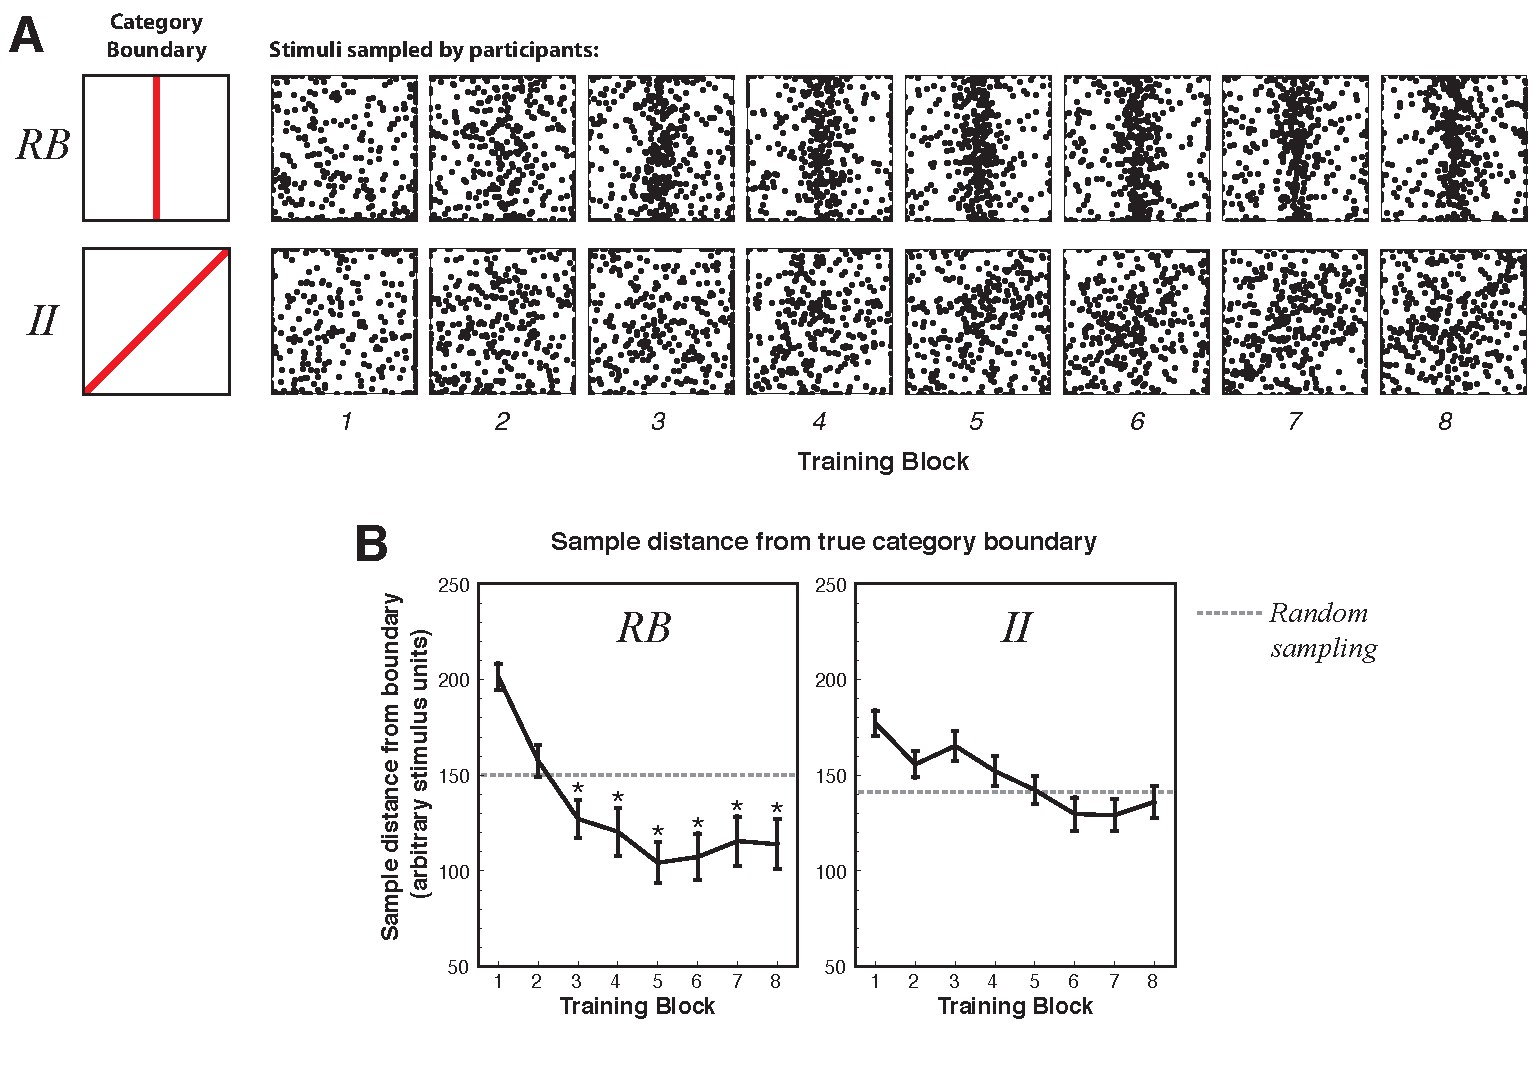
\includegraphics[height=4.5in]{figures/sampleplots.pdf}}
\caption{\textbf{A:} Distributions of samples chosen by self-directed participants in the RB (first row) and II (second row) tasks.  Each point in the plot specifies the size and angle of an antenna that a participant selected.  For purposes of illustration the stimulus spaces have been rotated so that the decision boundaries align.   \textbf{B:} Average distance of participants' samples from the optimal decision boundary by training block (black line). Dotted lines show the average distance expected from a random sampling strategy, and stars denote blocks in which sample distance was significantly smaller. In the RB task, participants sampled significantly closer to the true category boundary than expected by a random strategy by the 3rd block. In the II task, sample distance decreases over time, but never drops below the level expected from chance.  The difference in chance responding between the two tasks results from the orientation of the optimal decision boundary in the space.  Average sampling distances which appear ``worse" than random in the early blocks is the result of a bias that some participants showed toward sampling at the extreme edges of the space.  Error bars show the standard error of the mean.}
\label{sampledistance.fig}
\end{figure*}


While average sample distance decreased over time in both tasks, participants were clearly better able to sample along the true category boundary in the RB task than the II task. For example, in the RB task, average sample distance was significantly smaller than expected from a random sampling strategy (dotted lines in Figure~\ref{sampledistance.fig}B) by the third training block (one-tailed t-test, $t(28)=-2.21, p=0.017$) and in all subsequent blocks. In the II task, however, sample distance never dropped below the level expected from a random sampling strategy (one-tailed t-tests, all $p$-values $> 0.05$).


\subsection{Classification}
Responses during test blocks were scored according to whether the participant identified the correct category of each test item (as determined by the true category boundary). Two participants (one in the RB/Self-directed condition and one in the RB/Aware-yoked condition) were excluded from the analysis because their overall performance was at chance. Overall accuracy across tasks and conditions is shown in Figure~\ref{accuracy.fig}A. A 2-way ANOVA with task type (RB/II) and training condition (S/P/Y1/Y2) as between subjects factors found significant main effects of both task ($F(1,230)=226.4,p<0.001$) and training condition ($F(3,230)=5.59,p=0.001$), but no interaction ($F(3,230)=1.34, p=0.26$).


\begin{figure*}[t]
\centerline{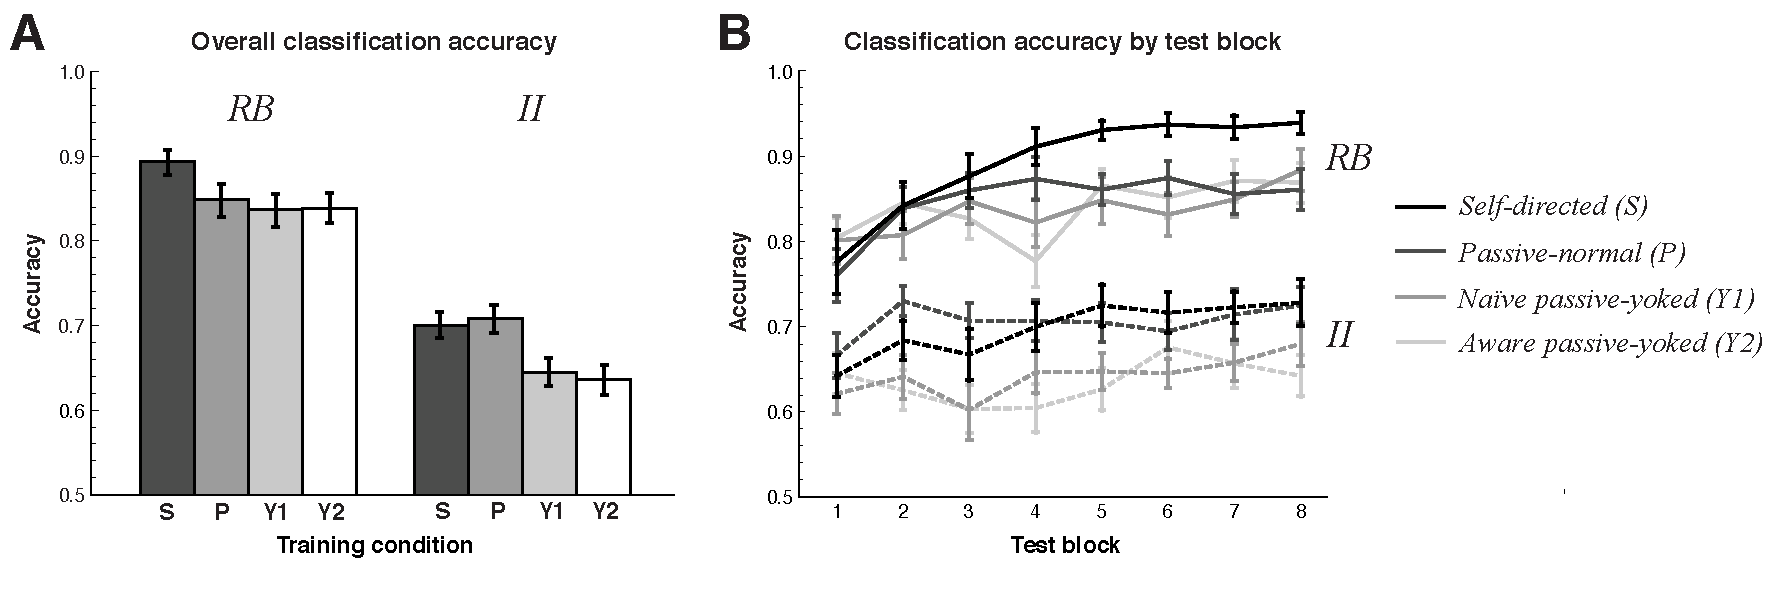
\includegraphics[height=2.4in]{figures/accuracycurves.pdf}}
\caption{\textbf{A}: Overall classification accuracy for each condition averaged across all test blocks. \textbf{B}: Mean accuracy for each condition as a function of test block (learners of the rule-based structure are depicted with solid lines, the II structure is shown as dashed lines). Error bars show the standard error of the mean in both plots.}
\label{accuracy.fig}
\end{figure*}


In the RB task, overall accuracy was marginally higher in the self-directed condition than in the passive-normal condition (P: $t(57)=1.82, p=0.07$), and significantly higher than both yoked conditions (Y1: $t(57)=2.33,p=0.02$; Y2: $t(56)=2.34,p=0.02$). There was no difference between accuracy in the passive-normal condition and either yoked condition (Y1: $t(58)<1$; Y2: $t(57)<1$), and no difference between the two passive-yoked conditions ($t(57)<1$). As shown in Figure~\ref{accuracy.fig}B, all four training groups perform at the same level in the early part of the task, but as the task progresses an advantage emerges for the self-directed learners over all three passive groups.  In the third block, the self-directed learners in the rule-based task already reached the same level of performance as the passive participants did in block 8 (see Figure~\ref{accuracy.fig}B).  Thus, it took the passive learners 2.66 times as long to achieve the same level of performance.

Within the II task, there was no difference between the self-directed and passive-normal groups ($t(58)<1$), but performance was greater in these two conditions when compared to either the Na\"{i}ve passive-yoked (S: $t(58)=2.46, p=0.02$; P: $t(58)=2.72, p=0.008$) or Aware passive-yoked (S: $t(58)=2.72, p=0.008$; P: $t(58)=2.97, p=0.004$). As in the RB task, there was no difference between the two passive-yoked training groups ($t(58)<1$).

Since passive-yoked group performance was lower than that of self-directed learners in both tasks, we were interested in whether individual PY participants benefited from being paired with high-performing self-directed participants. In both tasks, however, there was no correlation between self-directed learners' overall accuracy and the accuracy of passive-yoked learners linked to the same training data, regardless of whether the yoked learners were na\"{i}ve (RB: $r=-0.03, p=0.39$; II: $r=-0.11, p=0.33$) or aware (RB: $r=-0.08, p=0.36$; II: $r=-0.12, p=0.32$).

% RB naive: {-0.0323827, 0.389503}
% II naive: {-0.109441, 0.332012}
%
% RB aware: {-0.0835312, 0.360609}
% II aware: {0.122521, 0.319835}


We next tested whether there were differences in confidence ratings or reaction times during classification trials. 
While there was a main effect of task type (II learners were both less confident and slower to respond), there was 
no significant effect of training condition. Due to the lack of a difference between training conditions, confidence ratings and classification RT were not analyzed further.

%A separate two-way ANOVA was performed for each dependent measure (averaged across blocks). For confidence ratings, there was a significant main effect of task with confidence lower in the II task than RB task ($F(1,229)=46.5, p<0.001$), no effect of condition ($F(3,229)=2.35, p=0.07$) and no interaction ($F(3,229)=0.9$). Similar results were found for participants' classification reaction times, with a significant main effect of task type, with overall RT greater in the II task than RB task ($F(1,230)=4.86, p=0.03$), but no effect of training condition ($F(3,230)=1.82, p=0.14$) and no interaction ($F(3,230)<1$). 

%#             Df  Sum Sq Mean Sq F value   Pr(>F)    
%#task          1  27.703  27.703  46.562 7.85e-11 ***
%#cond          3   4.193   1.398   2.349  0.07332 .  
%#task:cond     3   1.605   0.535   0.899  0.44245    
%#Residuals   229 136.249   0.595                     

%#              Df    Sum Sq   Mean Sq F value  Pr(>F)  
%# task          1   5694657   5694657  4.8619 0.02845 *
%# cond          3   6394974   2131658  1.8199 0.14427  
%# task:cond     3   1374881    458294  0.3913 0.75940  
%# Residuals   230 269396495   1171289                  







%We next examined how the difference in accuracy between groups varied in different regions of the stimulus space. We measured the orthogonal distance of each test item to the category boundary and assigned them to four bins.  \\

%Error: subj
%     Df   Sum Sq  Mean Sq
%cond  1 0.060765 0.060765
%
%Error: subj:time
%     Df  Sum Sq Mean Sq
%time  1 0.18293 0.18293
%
%Error: Within
%                Df  Sum Sq Mean Sq  F value    Pr(>F)    
%cond             2  0.8577  0.4289  29.2702 6.133e-13 ***
%time             1  0.0840  0.0840   5.7354  0.016886 *  
%dist             1  5.6372  5.6372 384.7434 < 2.2e-16 ***
%cond:time        2  0.0285  0.0142   0.9711  0.379187    
%cond:dist        2  0.1434  0.0717   4.8926  0.007758 ** 
%time:dist        1  0.0803  0.0803   5.4816  0.019495 *  
%cond:time:dist   2  0.0101  0.0050   0.3431  0.709656    
%Residuals      706 10.3442  0.0147                       


%We next examined how accuracy changed in different regions of the stimulus space.  We divided the set of test items into two groups: those between the category means (thereby including the test items closest to the category boundary), and those outside of the category means. Separate 2-way ANOVAs were performed on participants' accuracy scores for test items in each of these regions. For items inside the category means, there were significant main effects of condition ($F(2,399)=8.14,p<0.001$) and block ($F(7,399)=9.60,p<0.001$), and a significant interaction ($F(14,399)=1.73, p<0.05$).  Pairwise tests on overall accuracy in this region revealed higher performance for active learners over passive ($t(38)=3.24,p<0.005$) and yoked ($t(38)=3.99,p<0.001$) learners, but no difference between passive and yoked conditions ($t(38)=0.79,p=.43$). For items outside the category means, there were significant main effects of condition ($F(2,399)=3.62,p<0.05$) and block ($F(7,399)=5.22,p<0.001$), but no interaction ($F(14,399)=1.44$).  Pairwise tests were consistent with the findings from above, showing an improvement for the active condition over the passive ($t(38)=2.46,p<0.05$) and yoked ($t(38)=2.89,p<0.005$) learners, while there was no difference between passive and yoked ($t(38)=0.32,p=0.75$). \\


%Error: subj
%     Df  Sum Sq Mean Sq
%cond  1 0.14254 0.14254
%
%Error: subj:time
%     Df  Sum Sq Mean Sq
%time  1 0.21712 0.21712
%
%Error: Within
%                Df  Sum Sq Mean Sq  F value    Pr(>F)    
%cond             2  1.4281  0.7140  28.3585 1.425e-12 ***
%time             1  0.1294  0.1294   5.1383  0.023706 *  
%dist             1  7.7920  7.7920 309.4705 < 2.2e-16 ***
%cond:time        2  0.0684  0.0342   1.3588  0.257633    
%cond:dist        2  0.1277  0.0639   2.5365  0.079864 .  
%time:dist        1  0.1956  0.1956   7.7698  0.005455 ** 
%cond:time:dist   2  0.1353  0.0676   2.6860  0.068850 .  
%Residuals      706 17.7761  0.0252                       



%For test items that fell between the category means, a 2-way ANOVA revealed a main effect of condition ($F(2,399)=2.55,p=0.08$) and a main effect of block ($F(7,399)=2.39,p<0.05$), but no interaction ($F(14,399)=0.91,p=0.55$). Followup tests showed the active group was significantly better than the yoked group ($t(38)=2.28,p<0.05$) but not the passive group ($t(38)=0.63,p=0.53$), while there was no difference between passive and yoked groups ($t(38)=1.57,p=0.12$).  For test items that were outside the category means, there were significant effects of condition ($F(2,399)=3.04,p=0.05$) and block ($F(7,399)=4.83,p<0.001)$), but no interaction ($F(14,399)=0.98,p=0.47$). Post-hoc t-tests on accuracy for test items outside the means again showed that the active group performed better than both passive ($t(38)=1.99,p=0.053$) and yoked ($t(38)=2.37,p<0.05$), but no difference between passive and yoked groups ($t(38)=0.26,p=0.79$).\\

\begin{figure*}[t]
\centerline{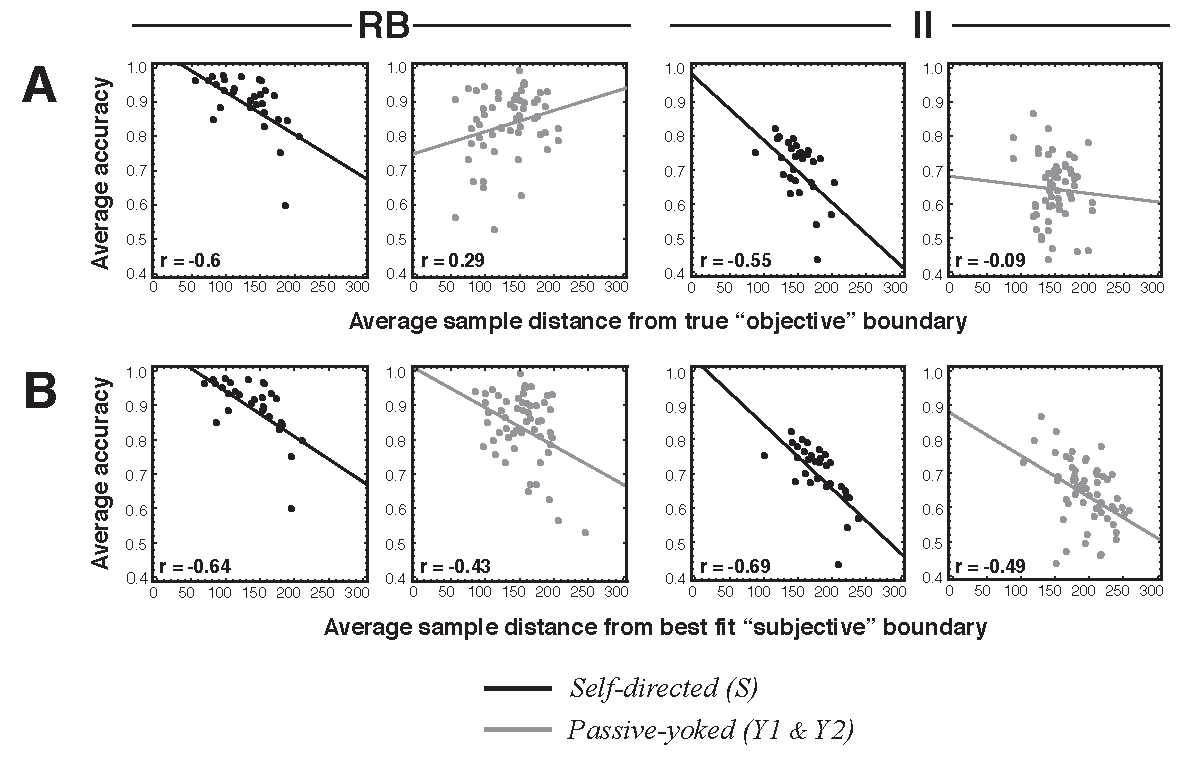
\includegraphics[height=3.5in]{figures/scatterplots_rev.pdf}}
\caption{
\textbf{A:} Relationship between the average distance of samples from the true category boundary and participants' overall accuracy, for both self-directed (black) and passive-yoked (gray) groups. Samples closer to the true boundary are associated with higher accuracy in self-directed but not passive-yoked learners. \textbf{B:} When sample distance is measured to a learner's best-fit boundary on the previous test block, it is correlated with overall accuracy for both self-directed and passive-yoked participants in both tasks.}
\label{scatterplots.fig}
\end{figure*}


% DOUG: this next part on study time is a good start, but doesn't really tell one too much actual information.  I think what we
%  want to do with 
% this particular analysis is attempt to rule out a story that active learning advantage comes from longer study times
% in that case we don't necessarily have to report all the stats or analyze it in this kind of omibus ANOVA way
% More to the point you could start this paragraph with the actual issue: Is the performance advantage just
% study time?  Then show that while self-directed too longer than others, the RTS were similar for both
% the RB and II tasks with a larger performance difference.  In addition, there were smaller, but robust differences
% between Y1 and Y2 despite being little difference in overall accuracy (and the same data!).  Thus, our results
% suggest that the learning performance differences are not straight-forwardly explained in terms of
% study time differences.  I guess my main suggestion is just to try to link it more to an issue in interpreting the data (help
% us rule out an uninteresting objection

%\subsection{Study time}
%One difference in the training procedure between the self-directed and passive conditions was the length of exposure to training stimuli. In the self-directed condition, manipulation of the stimulus was self-paced, followed by presentation of the category label for 1500ms. In all passive conditions, the stimulus was presented alone for 250ms, followed by the presentation of the category label, with the trial ending upon participants' verification of the label displayed. As a result, we expected there to be differences in the duration of training trials between conditions. A two way ANOVA on trial duration with task type (RB/II) and training condition (S/P/Y1/Y2) as between-subjects factors confirmed a significant main effect of training condition ($F(3,230)=115.9, p<0.001$), a main effect of task type (RB: $M=3148$, $SD=2110$; II: $M=3588$, $SD=2524$; $F(1,230)=5.2, p=0.02$), but no interaction ($F(3,230)<1$). As expected, trial duration was significantly greater in the self-directed condition ($M=6464$, $SD=1768$) as compared to all other conditions (P: $M=1846$, $SD=648$, $t(117)=16.76, p<0.001$); Y1: $M=2807$, $SD=1933$, $t(117)=10.76, p<0.001$; Y2: $M=2189$, $SD=999$, $t(116)=16.2, p<0.001$). There were also differences in trial duration between the three passive conditions; given their identical training procedures, these differences reflect the relative response time between passive groups. Passive-normal responses were faster than the Na\"ive yoked condition ($t(118)=-2.68, p=0.008$) but were not different from the Aware condition ($t(117)=-0.76, p=0.45$). Responses were significantly slower for Na\"ive passive-yoked than Aware passive-yoked participants ($t(117)=2.18, p<0.001$). Thus, while we found strong differences in trial duration between training conditions, the duration of stimulus presentation cannot account for the differences in classification accuracy previously described. Trial duration was significantly longer in the II task than RB task while accuracy followed the opposite pattern. Moreover, self-directed participants, on average, studied the training stimuli for a longer period of time than passive-normal participants in both tasks, but only performed better than that group in the RB task. \\
%


%#              Df    Sum Sq   Mean Sq  F value  Pr(>F)    
%# task          1  11522896  11522896   5.2076 0.02340 *  
%# cond          3 769976354 256658785 115.9923 < 2e-16 ***
%# task:cond     3    589969    196656   0.0889 0.96610    
%# Residuals   230 508926174   2212722                     


%Overall sample distance (averaged over blocks) was significantly smaller for participants in the RB task than in the II task ($t(57)=2.1, t=0.04$). While average sample distance decreased over time in both tasks, participants were clearly better able to sample along the true category boundary in the RB task than the II task. For example, in the RB task average distance was significantly smaller than the null hypothesis of a random sampling strategy by the third training block (dotted lines in Figure~\ref{sampledistance.fig}; one-sample t-test, $t(28)=2.21, p=0.04$). In the II task sample distance decreased over the course of training, but never dropped below the level expected from a random sampling strategy.\\

%            Df  Sum Sq Mean Sq F value    Pr(>F)    
% task         1   38115   38115 13.3331 0.0002903 ***
% block        1   58756   58756 20.5537 7.381e-06 ***
% task:block   1   14294   14294  5.0003 0.0258159 *  
% Residuals  466 1332127    2859                      


%## RB
%#t = 8.2908, df = 28, p-value = 1
%#t = 0.8963, df = 28, p-value = 0.8111
%#t = -2.2125, df = 28, p-value = 0.01763
%#t = -2.355, df = 28, p-value = 0.01288
%#t = -4.3714, df = 28, p-value = 7.707e-05
%#t = -3.5495, df = 28, p-value = 0.0006929
%#t = -2.9276, df = 28, p-value = 0.003357
%#t = -2.6829, df = 28, p-value = 0.006054
%
%## II
%# t = 5.4924, df = 29, p-value = 1
%# t = 2.1608, df = 29, p-value = 0.9804
%# t = 3.1275, df = 29, p-value = 0.998
%# t = 1.4372, df = 29, p-value = 0.9193
%# t = 0.173, df = 29, p-value = 0.5681
%# t = -1.31, df = 29, p-value = 0.1002
%# t = -1.4355, df = 29, p-value = 0.08092
%# t = -0.5907, df = 29, p-value = 0.2797


%%% DOUG : should we include another figure or panel that shows some of the individual data? that could be convincing for people.  or Perhaps we should at least mention some aspects of the individual data here?  i noticed in the discussion something says "notable exceptions" or whatever, so maybe should mention individual data?



\subsection{Relating sampling behavior and learning} Our next goal was to examine the relationship between sampling decisions and task performance. Specifically, we tested whether a participant's classification performance was related to how closely their training samples fell to the objective category boundary. For self-directed learners, we found that mean sample distance from the true category boundary was negatively correlated with overall test performance in both the RB ($r=-0.60, p<0.001$) and II ($r=-0.55, p=0.002$) tasks (see Figure~\ref{scatterplots.fig}A, black lines), showing that participants that sampled closer to the category boundary were more accurate overall. Interestingly, the same relationship was not found for passive-yoked learners who were trained with the same stimuli\footnote{Due to their equal test performance, Na\"ive and Aware passive-yoked groups were combined for this analysis. However, a similar relationship is found between sample distance and accuracy when the groups are considered separately.}. In the RB task, there was a positive correlation between sample distance and performance ($r=0.29, p=0.04$), while in the II task there was no correlation ($r=-0.09, p=0.3$). As is visible in Figure~\ref{scatterplots.fig}A, passive-yoked learners who received data which fell closer to the category boundary were among the worst performers in their group (particularly in the RB case) while this same training data was associated with higher performance in the self-directed participants. 

%RB
%Active: r=-0.603895 , p=0.000689751
%Yoked: r=0.286403 , p=0.0361559
%
%II
%Active: r=-0.545497 , p=0.00235944
%Yoked: r=-0.0961357 , p=0.302052


%One objection to measuring sample ``quality" by its distance from the true category boundary is that people may instead evaluate samples relative to their subjective belief about the boundary at any point in time.   Using logistic regression we found the best-fit linear decision boundary for subjects' response data on each test block. We then computed the average "subjective" sample distance from that boundary in the following training block, and computed the average over blocks for all active and passive-yoked participants. We found that this distance was smaller in the active group than passive-yoked group in both tasks highlighting the divergence in inference between the two groups (RB: $t(29)=-4.07, p<0.001$, II: $t(28)=-4.94 ,p<0.001$). In addition, subjective distance measure was negatively correlated with overall accuracy in all conditions (RB(A): $r=-0.54, p<0.005$, RB(PY): $r=-0.47, p<0.05$, II(A): $r=-0.79, p<0.001$, II(PY): $r=-0.41, p<0.05$, see Figure~\ref{sampledistance.fig}E).

%Given that subjective distance is correlated with performance in both active and passive-yoked training conditions, we next tested whether the main effect of training group remained after controlling for the distance covariate. An interaction between distance and training group might suggest that participants who observe highly informative samples do equally well regardless of training condition, but that passive-yoked participants who observe uninformative samples are impaired more than their active counterparts. However, a test of the homogeneity of slopes found no interaction between distance and training group ($\chi^2=$


%\noindent
%\textit{Active Sampling Behavior}\\
%Figure~\ref{sampling.fig} (top row) shows the distribution of queries for active learning participants in both the RM
%and II condition for the first and last training block.  In both conditions, participants begin by widely distributing
%their samples over the stimulus space.  However, by the eight training block, participant differentially allocate
%their samples to the area surrounding the true category boundary.  This is most pronounced in the rule-based
%task, but is also evident to a much weaker degree in the II condition.

%\begin{figure}[t]
%\centerline{\includegraphics[width=3.5in]{figures/sampling_kl.pdf}}
%\caption{\small{\textbf{Top row:} Samples chosen by participants in the active training condition for both block 1 and block 8
%and for the RB and II categories.  The color of the point denotes the category label feedback received on that sample. \textbf{Bottom row:} A map of the model's uncertainty over the feature space, as predicted by the \textit{KL divergence} sampling norm (averaged across 10 models trained on separate active participants). By the last training block, models trained on the RB task predict that the most useful queries will be centered on the true category boundary; in the II task, consistent with participants sampling strategy, the predictions of the model are less precise. }}
%\label{sampling.fig}
%\end{figure}


\subsection{Decision-bound analysis of test-block responses}  
In our final set of analyses, we attempted to characterize changes in participants' beliefs about the category boundary during learning.  Participants' current belief state is a latent variable.  However, to the degree that a participant's classification responses reflect their current understanding of the category, we can use these responses to infer the current belief about the category that the learner is considering. To this end, we fit linear decision boundaries to each participant's responses in each test block. Measuring changes in the parameters of the best-fit bounds from block to block provides a coarse description of the frequency and magnitude of shifts in beliefs over time. In addition, measuring sample distance from a participant's best-fit boundary (as opposed to the objectively true boundary) may be more informative about how self-directed sampling behavior relates to dynamic changes in the participant's belief state.

For each test block, a participant provides category labels for a set of items that are uniformly distributed throughout the stimulus space. We found the best-fitting linear decision boundary to explain each subject's pattern of responses in each test block.  Each unique decision bound can be described by three parameters: $\theta$, the angle of the decision bound in space; $b$, the bias, or offset, of the boundary from the center of the space; and $\sigma$, the determinism of the boundary. The likelihood that a given observation $o$ belongs to category A is a sigmoidal function defined by the parameters $\{\theta, b, \sigma\}$:

\begin{small}
\begin{equation}
P(o^t=A |  \theta, b, \sigma) = \frac{1}{1 + exp(-\sigma (o_1^t \cdot cos(\theta) + o_2^t \cdot sin(\theta)-b)}
\label{likelihood.eq}
\end{equation}
\end{small}

\noindent
where $o_i^t$ gives the observed value on dimension $i$ on trial $t$. Since the classification is binary, $P(o^t=B|  \theta, b, \sigma) = 1-P(o^t=A | \theta, b, \sigma)$. The likelihood of a particular set of labeled observations $\mathcal{D}=\{o^1, .., o^{n}\}$ is given by $P(\mathcal{D}|\theta,b,\sigma) = \prod_t P(o^t | \theta,b,\sigma)$. This basic model is equivalent to an equal variance Gaussian mixture model with two components. Given this likelihood function, the best-fitting parameters were found using a standard optimization procedure that maximizes the log-likelihood of each set of responses\footnote{Qualitatively speaking, most participant's test-block responses were well characterized by a linear decision boundary of this form.}.  These model fits were then used in the following set of analyses.\\

%However, for the minority of participants who responded using a more complex or heterogenous response strategy, this analysis provides less insight into their current category belief.


\subsubsection{Sample distance from best-fit ``subjective" boundary.} 
In our earlier analysis (Figure~\ref{scatterplots.fig}A), we used the distance of samples from the true category boundary as a measure of sample quality, and found that sampling closer to the boundary was associated with higher performance in self-directed, but not passive-yoked, learners. An interesting explanation of this divergence is that samples are useful only with respect to the learner's current beliefs.  Accordingly, the distance of samples from a learner's current ``subjective" decision boundary may better predict how they learn from those observations. To evaluate this idea, we measured the average distance of samples on each training block (excluding the first) to the best-fit decision boundary for the previous test block. Using this subjective measure, we again found that sample distance was strongly correlated with overall performance for self-directed learners in both tasks (see Figure~\ref{scatterplots.fig}B; RB: $r=-0.64, p<0.001$, II: $r=-0.69, p<0.0001$). Unlike the previous analysis, however, subjective sample distance was correlated with passive-yoked performance in both tasks as well (RB: $r=-0.43, p=0.02$, II: $r=-0.49, p=0.007$). A 2-way ANOVA on subjective distance with task and condition (A/Y) as between-subjects factors revealed significant main effects of both task ($F(1,172)=62.1, p<0.001$) and condition ($F(1,172)=8.42, p=0.004$), but no interaction ($F(1,172)<1$). In both tasks, subjective distance was smaller for self-directed learners than for passive-yoked learners (RB: $t(84)=-1.97, p=0.05$; II: $t(88)=-2.14, p=0.03$), as might be expected since self-directed learners were making the sampling decisions themselves. In addition, subjective distance was smaller in the RB task than II task, further suggesting that sampling is less effective in the II task.\\


\begin{figure}[t]
\centerline{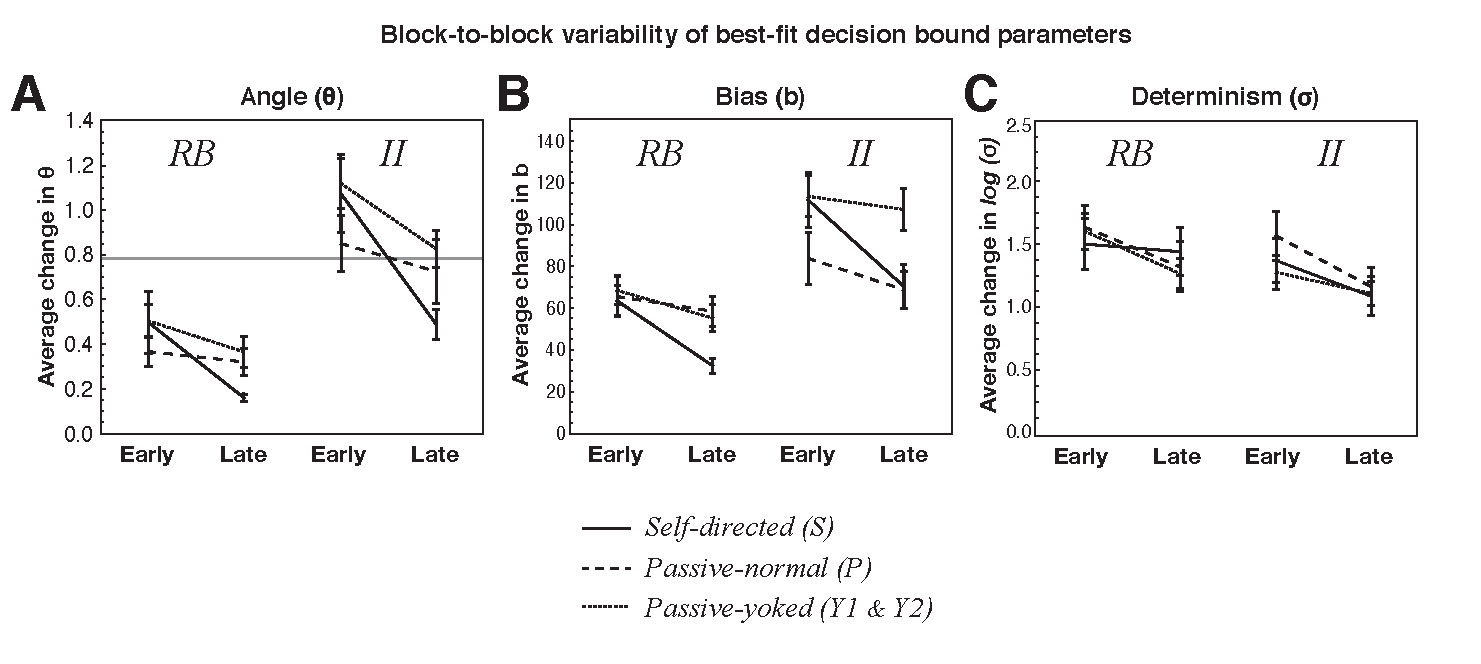
\includegraphics[height=2.8in]{figures/variability.pdf}}
\caption{Variability of best-fit decision bound parameters between test blocks (measured as average difference in absolute value of each parameter between subsequent blocks). Variability in both $\theta$ (\textbf{A}) and $b$ (\textbf{B}) was greater in the II task than RB task since participants were less successful at learning the diagonal rule. Variability between early blocks was the same for self-directed and passive-yoked participants. In late blocks, variability decreases more for self-directed than passive-yoked learners. Notably, in the II task the average change in $\theta$ for passive-yoked group in the second half of the task was approximately equal to a change from a uni-dimensional rule to a diagonal rule (marked by the dotted line). \textbf{C:} Variability in the best-fit value of $\sigma$ (transformed to log scale) is higher in the RB task than II task, but there are no differences between self-directed and passive-yoked learners.}
\label{variability.fig}
\end{figure}



\subsubsection{Variability in classification strategy during learning.} Measuring changes in the best-fit parameters from block-to-block gives a coarse description of how beliefs about the category boundary are changing over time. For example, given that $\theta$ describes the importance attributed to either feature dimension, changes in $\theta$ signal exploration of different forms of rules. Changes in $b$, on the other hand, suggest refinement of the location of the boundary in space (although changes in both parameters can occur simultaneously). Variability in the value of $\sigma$, unlike the other two parameters, does not reflect adjustments to the location of the boundary in space but rather changes in the determinism of responses. 


The magnitude (i.e., absolute value) of changes in best-fit parameters was measured between pairs of consecutive test blocks and averaged across early ($1\rightarrow2$, $2\rightarrow3$, $3\rightarrow4$) and late ($5\rightarrow6$, $6\rightarrow7$, $7\rightarrow8$) transitions. Since the distribution of these values violated the assumptions of standard t-tests, we used the non-parametric Wilcoxon rank sum test to evaluate differences in variability between conditions. Figure~\ref{variability.fig} provides a compact summary of these analyses.  First, consider the variability of $\theta$ (Figure~\ref{variability.fig}A) and $b$ (Figure~\ref{variability.fig}B). Overall, variability in both parameters was greater in the II task than the RB task ($\theta$: $W=11878, p<0.001$, $b$: $W=1191, p=0.012$). This suggests that II learners were more likely to make large changes to their classification decision strategy from one block to the next.

Focusing now on the RB condition, in the first half of the task, there is no systematic difference in the variability of either $\theta$ and $b$ between conditions. In the latter half of the task, however, variability in the same parameters is significantly lower in the self-directed condition that both passive training conditions (P: $W=296, p=0.03$, Y: $W=575, p=0.01$), while variability is not different between passive-normal and passive-yoked conditions. Thus, by the second half of the RB task, self-directed participants have learned the correct form of the rule and make smaller adjustments from block to block than participants in the passive conditions.

Variability of $\theta$ and $b$ in the II task follow a similar pattern for the self-directed and passive-yoked conditions. The major difference in this task is that passive-normal learners show less variability in $b$ in early blocks than the other conditions (S: $W=605, p=0.02$, Y: $W=1170, p=0.02$), and equal variability to the SD condition in late blocks for both $\theta$ and $b$ (consistent with their classification performance being the same as the SD condition).

%In the first half of either task, self-directed and passive-yoked learners show no difference in the variability of both $\theta$ (RB: $W=703, p=0.17$; II: $W=805, p=0.42$) and $b$ (RB: $W=849, p=0.95$; II: $W=903, p=0.98$). In the latter half of both tasks, however, variability is significantly lower in the self-directed condition than passive-yoked group, again for both $\theta$ (RB: $W=575, p=0.01$; II: $W=599, p=0.01$) and $b$ (RB: $W=601, p=0.02$; II: $W=601, p=0.01$). 

Variability in $\sigma$ (see Figure~\ref{variability.fig}C) indicates differences in how deterministic responses were from block to block (e.g., transitioning from random classification on one block to the use of a sharp, deterministic rule on the subsequent block). Overall variability in $\sigma$ (transformed to log scale) was significantly higher in the RB task than II task ($W=31330, p=0.045$). However, there were no differences in the variability of $\sigma$  between training conditions in either early or late blocks. 
%Thus, while variability in $\sigma$ may be related to the overall difference in performance between category structures, it seems unrelated to the divergence between self-directed and passive learners.

The key point from this analysis is that poorer performance for the passive conditions in the RB task and the PY group in the II task is related to ongoing search for the correct form of decision boundary.  In particular, the pattern suggests that passive-yoked behavior is marked by larger, more frequent shifts in decision bounds throughout the experiment (as may be expected from sequential hypothesis testing). Notably, the average change in $\theta$ for passive-yoked learners in the latter half of the II task is approximately equal to a shift from a uni-dimensional rule to a diagonal rule (marked by the gray line in Figure~\ref{variability.fig}A), reflecting their inability to learn the simultaneous relevance of both feature dimensions. In contrast, changes in both $\theta$ and $b$ are smaller in late blocks for self-directed learners, consistent with their higher overall accuracy. 






%% RB
%Active: r=-0.635162 , p=0.000285854
%Yoked: r=-0.434915 , p=0.0209916

%% II
%Active: r=-0.692858 , p=0.0000300922
%Yoked: r=-0.494669 , p=0.00675753


%             Df Sum Sq Mean Sq F value    Pr(>F)    
%task          1  71327   71327 62.0791 3.592e-13 ***
%cond          1   9677    9677  8.4227  0.004191 ** 
%task:cond     1      1       1  0.0006  0.981105    
%Residuals   172 197622    1149                      

% RB
% t = -1.9669, df = 84, p-value = 0.0525
%
% II
% t = -2.1445, df = 88, p-value = 0.03475





\section{Discussion}
There are a number of key observations from the experiment. First, we found a main effect of category structure, with participants in the II task performing more poorly overall, consistent with previous studies that used a similar form of observational learning~\citep{Ashby:2002p13331}. Although self-directed learners in the II task out-performed both passive-yoked groups, they were unable to achieve accuracy comparable to RB participants. In addition, their sampling behavior suggests that most self-directed learners in the II condition were unable to sample along the diagonal category margin (although inspection of individual subject data revealed a few highly effective II samplers, showing that such sampling was not impossible). In contrast, self-directed learners in the RB task preferred samples close to the true category boundary. It is notable that participants with no knowledge of the abstract category structure were able to sample effectively, supporting previous findings of efficient sampling in other tasks~\citep{Castro:2008p12850,Oaksford:1994tw}.

Secondly, self-directed learners were more accurate than passive-normal participants in the RB task. One explanation for this difference is that self-directed learners were able to query regions in the stimulus space where they were most likely to commit classification errors (i.e., near the category boundary). Since participants in the passive-normal condition received samples from fixed category distributions, they were less likely to observe training items close to the critical boundary. In contrast, self-directed learners in the II task were less likely to sample from the true category margin and had lower accuracy than the same condition in the RB task.  
%\hl{Keep in mind that the advantage for self-directed sampling could have conceivably been opposite (people might have been unable to learn the category when they designed their own training example).

However, any advantage for self-directed learners cannot be explained by a difference in training data alone. Most striking is the finding that yoked participants were less accurate than the self-directed group despite learning from the exact same observations. Indeed, the passive-yoked participants who observed what might be considered the most objectively useful training data (as measured by distance from the true category boundary) were among the worst performers, particularly in the RB task. If self-directed and passive-yoked learners are assumed to update their beliefs through a common process (as would be predicted by existing models of human categorization) then this strong pattern of divergence is unexpected. In the following section, we present a model-based analysis of these effects.

Finally, the results of the decision bound analysis provide insight into the basis for participants' errors during learning. For example, it is not the case that passive-yoked learners fail to classify items systematically or to change their beliefs following poor performance in a test block.  Instead, their response variability suggests that, on the whole, passive-yoked participants continue to search for the correct decision bound but are less likely to acquire (and maintain) it than self-directed learners. Overall, our data is consistent with the idea that participants were engaged in sequential hypothesis testing~\citep{Bower:1964kn,gregg1967process,Nosofsky-1994ck,nosofsky1998rule}.

The large changes in response strategy from one block to the next are in need of additional explanation. Given the simplicity of the binary classification task, even a small number of observations is usually enough to constrain the location of the decision boundary (e.g., the boundary must fall somewhere between the two nearest examples of each category).  However, even in the second half of the task, we found that some participants flipped which dimension they were using to classify exemplars, particularly in the yoked conditions.  This is unexpected if participants were integrating over all previous training examples.  One possible explanation for this response variability is that participants only use a small number of recent observations to evaluate their belief about the category rule (consistent with the classic studies of hypothesis testing by Bower and Trabasso, 1964). This fact is also intuitively likely given that the category exemplars are highly similar to one another and easily confusable.  Ultimately, a limited memory for recent examples may heighten the importance of ``good" sampling throughout the task, such that the most recent examples are used to judge the validity of the learner's existing belief about the category boundary.
 \nocite{Bower:1964kn}
 
%This interaction of memory constraints and sample quality may help to explain gaps in performance between groups with identical training sets but divergent hypotheses, and is the subject of the model described below. 




% \begin{figure}[t]
%\centerline{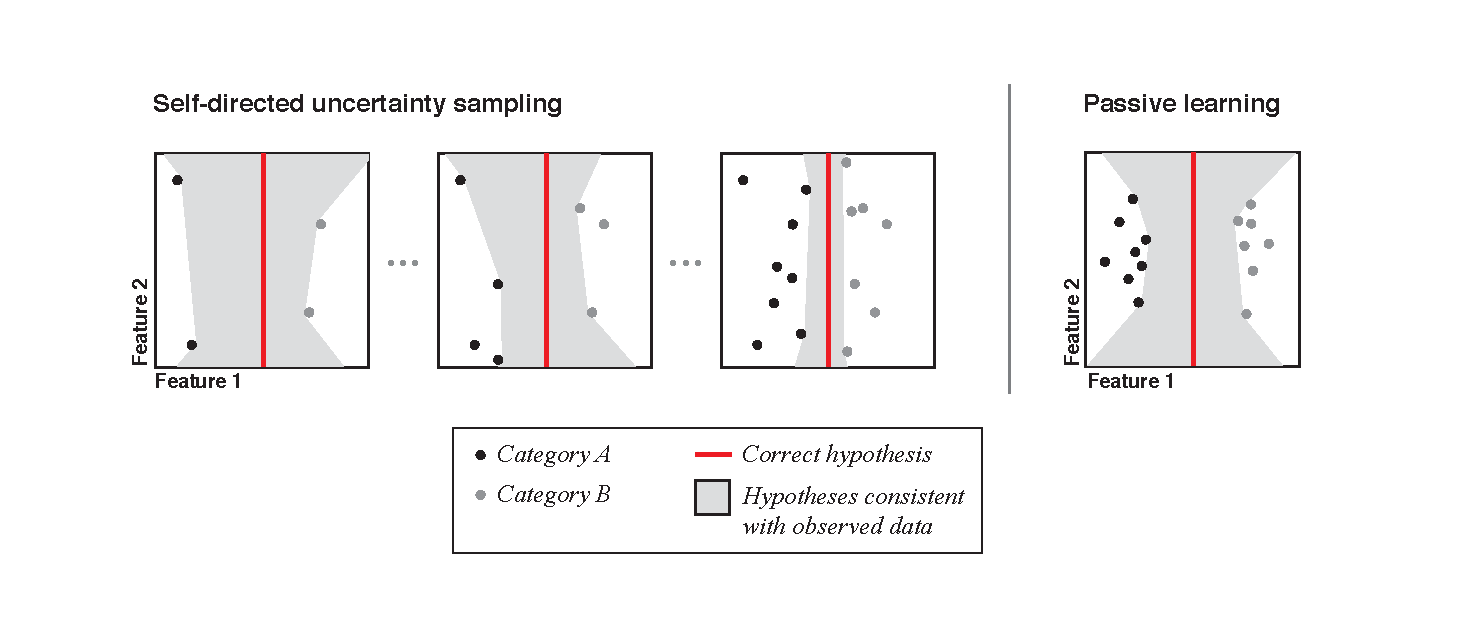
\includegraphics[width=6in]{figures/setup.pdf}}
%\caption{\textbf{A:} Self-directed sampling in the region of uncertainty. \textbf{B:} Passive learning is limited by the samples provided by the environment.}
%\label{activelearning.fig}
%\end{figure}

% Figure~\ref{activelearning.fig} depicts the general problem for learning a linear classification boundary. Given an unknown boundary between classes (shown by the vertical line), the objective is to sample a new observation that will be informative about the category structure. A common way to judge an item's information value is to use the classifier's uncertainty about how to label it as a measure of how useful it will be to query that item (e.g., previously observed items have low value and items that might belong to either category have high value). In this case, since there are many potential category boundaries that could have given rise to past observations, uncertain items are those that fall in the region defined by that set of hypotheses (depicted by the gray area). As more data is collected the space of possible hypotheses shrinks and the set of informative observations will become clustered close to the true category boundary (note that in a \emph{passive} learning situation the data distribution is not controlled by the learner, and a similar reduction in uncertainty may never occur). 
%
%If human learners use their uncertainty in an analogous way, successful sampling should follow the same pattern. Each individual may begin a category learning task with a different belief about the classification rule (e.g., a randomly chosen linear boundary). The learner samples new data to test their current hypothesis, which may then change in response to those observations. Over the course of learning, as their belief converges on the true category boundary, samples should be increasingly drawn from the margin of the true category boundary. This process of sequential hypothesis testing embodies previous findings of ``rational" information sampling in reasoning~\citep{Oaksford:1994tw} and classification~\citep{Nelson:2005ph}. 
%
%Of course, there is reason to expect that human learning may diverge from the predictions of optimal sampling models. For example, unlike an artificial classifier, people have a well-documented bias toward unidimensional rules, and indeed may learn more complex rules using separate cognitive processes~\citep{Ashby:1999ig,Ashby:1998p8468}. As a result, the ability to generate hypotheses and collect useful data may depend on the form of the particular concept being learned. A failure to sample may compound prior biases and inhibit learning, since the person is unable to collect data that will be informative about the target concept. The model we will describe has much in common with existing accounts of rule learning in similar categorization tasks (e.g., RULEX, \citet{nosofsky1998rule}; or COVIS, \citet{Ashby:2010p14184}), but makes a novel contribution by describing this interaction of prior biases with information sampling.


\section{A model of sequential hypothesis generation and information sampling}

In this section we describe a formal model of how the interaction between self-directed information sampling and learning can explain our experimental results.  At the broadest level, our theory asserts that people engage in sequential hypothesis testing during learning (consistent with the ongoing shifts in response rules seen in the experiment as well as existing work on category acquisition), and that currently active hypotheses serve as the basis for sampling new observations during learning. 

In our simulations, we address two theoretical challenges posed by the behavioral results. First, given the focus placed on passive learning in the literature, existing category learning models provide no explicit account of how self-directed sampling might affect acquisition. In Simulation 1 we show that our mechanistic information-processing model is capable of recreating the pattern of results across training conditions, without assuming any differences in the learning process or parameters between the self-directed and passive groups. 

Second, existing models have difficulty explaining the divergence between self-directed and yoked learners (since the sequence of training examples was identical in both conditions). 
Importantly, simply assuming that self-directed learning is advantageous because of generally increased ``engagement" would not account for the systematic interaction between sampling behavior and classification performance (i.e., under a generalized ``engagement" hypothesis Figure \ref{scatterplots.fig} would show a main effect rather than an interaction). Our second simulation tests our hypothesis that this relationship is a direct consequence of the hypothesis-testing process that is central to the model.


%Our results raise a number of interesting challenges for existing theories of human category learning.
%First, given the focus placed on passive learning in the literature, existing models provide no explicit 
%account of how participants might make information sampling decisions in the self-directed 
%learning condition.  

%Second, most existing models have difficulty explaining the systematic divergences between the self-directed and
%yoked learners (since the sequence of training examples was identical in both conditions). In this section, we present a process-level account of learning that builds on common features of existing theories to explain our behavioral findings. 

%In general, our approach assumes that people engage in sequential hypothesis testing during learning (consistent with the rapid shifts in response rules seen in the experiment), and that their hypotheses serve as the basis for sampling new observations during learning. Our overall approach derives directly from principles of rational Bayesian inference, but under the assumption that the learner has limited resources for representing alternative hypotheses~\citep{brown2009detecting}.\\

\subsection{Description of the model}
Our model is based on five simple, interacting principles.  First, we assume that the learner's category representation takes the form of probabilistic decision rules.  Second, we assume that people generate new hypotheses on each trial based on a stochastic search processes.  Third, we assume that this search process is strongly biased by a prior toward simple, unidimensional (i.e., axis-orthogonal) rules.  Fourth, we assume that only a limited number of prior training examples influence participant's current response strategy (i.e., a bias toward recent observations).  Finally, we assume that self-directed participants actively gather observations which they are currently uncertain how to classify.   Each of these assumptions is motivated by prior literature of human categorization, key aspects of our empirical data, and realistic psychological constraints.   Together, these principles (described in detail below) interact to drive our key predictions about performance in the task.

\subsubsection{Category representation}
We assume that learners classify items using simple decision rules~\citep[similar to][]{nosofsky1998rule,Ashby:2010p14184}.
The goal of learning is to infer the rule which correctly classifies the most
items.  Formally, each hypothesis about the true category rule
is represented as a probabilistic, linear decision bound which assigns a probability 
of category membership to each item 
in the space using Equation~\ref{likelihood.eq}.  An individual hypothesis
is defined by two parameters, $\textbf{h}_m^t=(\theta_m^t,b_m^t)$, which control the position and orientation of the decision boundary in the stimulus space (for simplicity, we assume all hypotheses have the same determinism, specified by $\sigma_0$, a free parameter). 
%(Notice that each hypothesis in the model corresponds 
%directly to the decision-bound model used in our earlier data analysis.)
Given this representation of categorization rules, an ideal Bayesian learner
would estimate the posterior probability of each possible hypothesis given a 
suitably defined prior over the parameters of the 
space and a set of observations, $D$ ~\citep[see][for a similar approach]{Courville:2003rm}:

\begin{equation}
p(\textbf{h}_m^t|D) \propto p(D|\textbf{h}_m^t)p(\textbf{h}_m^t)\label{posterior.eq}
\end{equation}
 
\noindent
This computational-level description of the
learning problem helps expose the relationship between our approach and recent Bayesian models
of cognition~\citep{Griffiths:2010fk}.
However, given capacity limitations, it is unlikely that participants can simultaneously
update and represent this entire hypothesis space~\citep{Vul:2009xi,brown2009detecting}.  Instead, we assume that participants
maintain a limited set of $M$ hypotheses in memory at any point in time.  In fact,
in the subsequent simulations, we place an extreme constraint on this by assuming the
learner represents just a single ``active" hypothesis at any point in time ($M=1$), which is 
used as the basis for classification and sampling decisions.  Increasing the capacity of 
the model ($M \rightarrow \infty$) leads to a richer representation of the posterior while increasing the 
computational demands of learning \citep{Sanborn:2006p9933}.  Such approximate Bayesian techniques
are referred to as ``rational process models"~\citep{Vul:2009uq}.\\

\subsubsection{Generating new hypotheses}
Consider a learner that represents a single
hypothesis about the category described by 
parameters $\textbf{h}^t=(\theta^t,b^t)$ on trial $t$.  On each
trial of the learning task, we assume that the learner considers making a change to the current
hypothesis.  The stochastic procedure for this is as follows.  First, one of the two 
parameters is randomly selected and used to generate a proposal, $\textbf{h}'$.  This proposal is 
essentially a local change to the form of the current hypothesis.  In general, a new value for
the selected parameter is sampled from 
a Gaussian distribution centered on the current value of the parameter 
($\theta' \sim N(\theta^t,s_{\theta}); \hspace{.05in} b' \sim N(b^t,s_b))$. 
The remaining parameter value in $\textbf{h}'$ is unchanged 
from the current hypothesis.  By this mechanism, very local changes to the hypothesis
are made at each point in time. However, consistent with our data, we assume that subjects are willing to consider more radical changes to the form of their hypothesis. To accommodate such changes, we assume that when $\theta$ is selected as the parameter to change, with probability $p_\theta$ the learner will instead draw a proposal directly from their prior (defined below). 

%However, consistent with our data, we assume that
%subjects sometimes are willing to consider more radical proposals.  To accommodate such
%changes in the model, we assume that when $\theta$ is selected as the parameter to
%change, with probability $p_\theta$, the learner will instead draw a proposal for $\theta$
%directly from their prior (defined below).  

\begin{table}[t]
\caption{Settings of model parameters}

\begin{tabular}{r|c}
\textbf{Parameter} & \textbf{Value} \\
\hline
Number of active hypotheses: $M$ & 1 \\
\hline
Number of observations: $n$ & 5  \\[1.1ex]
\hline
Prior weights: $\alpha$ & 0.05 \\ 
$\beta$ & 0.05  \\[1.1ex]
\hline
Width of proposal distributions: $s_{\theta}$ & $\pi/4$ \\
$s_b$ & 20 \\
\hline
Rule determinism: $\sigma_0$ & 0.1 \\
\hline
Probability of sampling $\theta$ from prior: $p_\theta$ & 0.5 \\
\end{tabular}
\label{par.fig}
\end{table} 

After a proposal has been generated, the learner either adopts or rejects it based on the \textit{acceptance ratio}, the relative likelihood of the existing and proposal hypotheses (given by the unnormalized posterior probability estimates $P(\mathcal{D}|\textbf{h}^t)$ and $P(\mathcal{D}|\textbf{h}')$). If the proposal hypothesis provides a better account of the data (i.e., if $P(\mathcal{D}|\textbf{h}')/P(\mathcal{D}|\textbf{h}^t) > 1$), the proposal is accepted as the new active hypothesis $\textbf{h}^{t+1}$. If the new hypothesis results in a worse account of past data, it is still accepted in proportion to the acceptance ratio; otherwise the current parameter estimate remains unchanged. This procedure is known as the Metropolis-Hastings algorithm, a form of Markov-Chain Monte Carlo~\citep{Metropolis:1949ri}.
%\footnote{Interestingly, using this simple rule, the frequency with which each hypothesis will be
%considered will approximate the true posterior distribution over all hypotheses (in the limit).}.  



The psychological demands of this procedure are low and quite plausible: on each trial, the learner must simply generate a new hypothesis and judge its quality relative to a single existing hypothesis.  Sometimes a proposal is accepted and the current hypothesis changes, and other times it is rejected as being a worse account.  As mentioned above, we begin with the simplest possible assumption in that the learner considers only a single hypothesis on every trial, but the framework is general enough to accommodate parallel updating of multiple hypotheses in separate ``chains." \\


%After a proposal has been generated, the learner is assumed to compare this new proposal to the existing hypothesis and ``accept" it as the active hypothesis $\textbf{h}^{t+1}$ if it provides a better account of the data (i.e., if $P(\mathcal{D}|\textbf{h}')>P(\mathcal{D}|\textbf{h}^t)$ then $h^{t+1}=h'$). 

%given by the unnormalized posterior probability estimate for that hypothesis, $P(\mathcal{D}|\textbf{h}')$). 

%At a given point in time we assume
%the learner has in mind a decision rule which can be characterized by parameter set
%$p^t=\{\textbf{w}^t, b^t, \sigma^t\}$.  On each trial, a new set of parameters $p^{t+1}$ is proposed (or
%generated) which represents a change to the current rule.  The learner is assumed to compare
%this new hypothesis to the old one and ``accept" it as the new hypothesis 
%if it provides a better account of the data (weighted by the prior belief in that parameter 
%combination).  If the new hypothesis results in a worse account of past data, it is accepted in proportion to the relative posterior likelihood of the new hypothesis compared to the old, otherwise
%the current parameter estimate remains unchanged. This procedure is similar to the Metropolis-Hastings algorithm (a form of Markov-Chain Monte Carlo) with an additional parameter $k$ dictating the likelihood of accepting a proposal with a lower posterior estimate, giving the acceptance function $P(\mathcal{D}|p^{t+1})/(P(\mathcal{D}|p^{t}) + k)$. Proposals were generated from independent Normal distributions centered on the current parameter estimates: $\textbf{w}^{t+1} \sim N(\textbf{w}^t,\pi/2); \hspace{.05in} b^{t+1} \sim N(b^t,20); \hspace{.05in} \sigma^{t+1} \sim N(\sigma^t, .05)$. The computational demands of this procedure are low: the learner is assumed to maintain a single hypothesis at any point in time. On each trial they must simply generate a new hypothesis and judge its relative quality. While we began with the simplification of assuming that the learner considers a single hypothesis on every trial, it is also possible that participants consider multiple hypotheses which are simultaneously updated in the same way. \\


%While there have been a number of models proposed for how people classify
%items using rules in continuous dimension spaces, there have been fewer attempts to articulate an
%inference procedure for such models (cf. ~\citep{Nosofsky:1998yy}).  As a result,
%there were two key properties that guided the development of our modeling framework.  First,
%we wanted a way to specify a strong inductive bias towards uni-dimensional rules along
%either stimulus dimension (similar to the default verbal system in~\citep{Ashby:1998oa}).  Most existing models can specify a prior bias towards a particular 
%dimension (e.g., based on salience), but not a more 
%general preference for arbitrary uni-dimensional rules~\citep{heller2009dimensionalbias}.  Second, analysis of the decision 
%rules that participants use from one block to the next suggested that these were updated 
%in a rather rapid fashion characteristic of serial hypothesis testing.

%These concerns led us to a probabilistic model of
%classification which assumes that the goal of learning is to discover the
%latent parameters of a simple linear decision boundary.    
%In our model, the probability that an observation, $o^t$, on
%trial $t$ falls in category A is assumed to depend on a set of latent model parameters $\{\textbf{w}, b, \sigma\}$:
%\noindent
%where $o^t_i$ is the stimulus value of dimension $i$.  Since the classification is binary, $P(o^t=B|  \textbf{w}, b, \sigma) = 1-P(o^t=A | \textbf{w}, b, \sigma)$.
%The weight vector, $\textbf{w}$, contains the decision weight assigned to each dimension.  The bias
%term, $b$, allows fine adjustments to the position of the decision rule in the stimulus space.  Finally, the slope of the sigmoid function is controlled by $\sigma$ which reflects how deterministic 
%the decision rule is.  Thus, each parameter combination
%$\{\textbf{w}, b, \sigma\}$ reflects a unique decision rule or hypothesis about the category.  The likelihood
%of a particular set of labeled observations $\mathcal{D}=\{o^1, .., o^{t}\}$ is given by $P(\mathcal{D}|\textbf{w},b,\sigma) = \prod_t P(o^t | \textbf{w},b,\sigma)$ (see~\citep{Courville:2003rm} for a similar approach).
%This basic model is equivalent to an equal variance Gaussian mixture model with two components.
%\textit{Uni-dimensional bias}. We assume that learners are strongly biased toward unidimensional rules along either dimension.  Accordingly, we defined a prior over the decision weights $\textbf{w}=\{w_1=cos(\theta),w_2=sin(\theta)\}$, where $\theta$ is the angle of the vector corresponding to the decision boundary.   We created a piece-wise scheme for


\subsubsection{Prior}
We assume that learners are strongly biased toward unidimensional rules along either dimension.  Accordingly, we defined a prior over $\theta$, the angle of the vector corresponding to the decision boundary, which favored axis aligned rules \citep[cf.][]{Heller:2009fk}.  We created a piece-wise scheme for translating $\theta$ into relative distance $r$ from the orthogonal axes (bound between 0 and 1):
\begin{equation}
   r= \left\{
     \begin{array}{ll}
       (2 \theta)/\pi & : 0 < \theta \le \frac{\pi}{2}\\
       (2 (\pi-\theta))/\pi  & : \frac{\pi}{2} < \theta \le \pi\\
       (2 (\theta-\pi))/\pi  & : \pi < \theta \le \frac{3\pi}{2}\\
       (2 (2\pi-\theta))/\pi  & : \frac{3\pi}{2} < \theta \le 2\pi\\
     \end{array}
   \right.
   \label{priorcode.eq}
\end{equation} 
with the prior distribution: 
\begin{equation}
r \sim Beta(\alpha,\beta)
\end{equation}
Using this form, $\alpha$ and $\beta$ act as a type of abstract decision weight for the two stimulus dimensions. When $\alpha=\beta < 1$, there is a general preference for axis-orthogonal rules that involve only a single dimension (see Figure~\ref{simresults.fig}A). On the other hand, $\alpha=\beta=1$ implies no preference for rules of a particular orientation.  This choice of prior (specifically $\alpha,\beta<1$) is consistent with a large body of empirical and theoretical work suggesting that learners find axis-aligned boundaries easier to learn and are biased to use such rules early in learning~\citep{Ashby:1998p8468,Ashby:1999ig,Ashby:2002p13331}\footnote{Specifically, our approach is most similar to COVIS~\citep{Ashby:1998p8468}, in which an explicit rule-generating system competes with an 
implicit exemplar-based system to produce responses. Importantly, people are assumed to rely 
initially on the explicit system, with a strong bias toward using uni-dimensional rules for classification. 
One source of evidence for this bias is typical behavior in the II task, in which early responses are best 
fit by suboptimal, uni-dimensional decision boundaries, and learning of the correct II boundary emerges 
slowly over the course of training~\citep{maddox2004dissociating}. Given the relatively small amount of training data and the use of observational training in our II task, our results likely reflect an early stage of learning in which participants primarily rely on simple rules~\citep{Ashby:2002p13331}.}. The prior over the bias term was a uniform distribution over the stimulus space.  \\



\subsubsection{Limited Memory} 
As mentioned in the discussion of our empirical results, our analysis of how participants changed their decision rules over the course learning suggested that learners typically do not optimally
integrate past training episodes into their decision strategy.   Optimal integration is specifically contradicted by large changes in the form of the decision rule even late in training.    

To capture this aspect of our data, we allowed for the possibility that learners store only $n$ recent observations in memory (a free parameter that we fit in our simulations), and evaluate the likelihood of a hypothesis with respect to this limited set.   This assumption is intuitively plausible given how perceptually similar the training examples were and how many distinct stimuli are present in the task.

This capacity limitation for previous training examples results in ongoing shifts in the currently estimated decision rule, consistent with the variability in participants' response behavior throughout the task.  Given the strong prior favoring rules along a single dimension, the estimate of $\theta$ will tend to bounce between the different modes of the hypothesis space, and convergence on the correct mode will depend on the informativeness of recent training samples.   Note that without the assumption of limited capacity for previous examples, the model will rarely switch decision strategies after the first few training examples and will tend to learn much more quickly than human participants.\\

\subsubsection{Self-directed Information Sampling} 
Finally, we assume that self-directed learners preferentially select observations which they are currently uncertain about how to classify.  This hypothesis is supported by our empirical results in Figure~\ref{sampledistance.fig} and~\ref{scatterplots.fig}B which show evidence of preferential sampling of examples near the learner's current estimate of the boundary between the two categories.  Such uncertainty-driven information sampling is also largely consistent with recent theories of rational information acquistion~\citep{Oaksford:1994tw,Nelson:2005ph}. Formally, the model's uncertainty about a new observation $x$ is calculated using \textit{label entropy} (LE):

\begin{equation}
LE(x)=-\sum_{l \in \{A,B\}} P(x=l |  \textbf{h}^t) \; log \; P(x=l | \textbf{h}^t)
\label{labelentropy.eq}
\end{equation}

\noindent
Label entropy measures the relative value of a sample based on the model's certainty in its category label $l$. Items are preferred when both the category A and B labels appear to be equally plausible (i.e., the learner is highly uncertain) and items are avoided when the belief in one label strongly dominates the other\footnote{As noted by Nelson (2005), almost all measures of information value make the same prediction that items near the learner's current boundary should be preferred.  Label entropy thus represents one hypothesis about how new observations might be valued.  Differentiating various ways that people might make these decisions is the focus on ongoing work.}.   In our simulations, this value was calculated for a uniform grid of points $X$ in the space, and converted to choice probabilities using the softmax choice rule~\citep{Sutton:1998lr}:

\begin{equation}
p(o^t=x|\textbf{h}^t) = \frac{e^{d \cdot LE(x)}}{\sum\limits_{x' \in X}^{} e^{d \cdot LE(x')}}
\label{choiceprob.eq}
\end{equation}

\noindent
Items are then sampled in accordance with these choice probabilities.  The $d$ parameter specifies the \textit{sampling determinism}, or the randomness of sampling behavior. When $d=0$, samples are generated randomly over the entire space; when $d$ is high, samples are biased toward points with greater label entropy. As a result, a higher value of $d$ produces samples closer to the currently hypothesized decision bound. \\

% DOUG: this figure is great, but the caption still doesn't explain it clearly enough.  i'd start with defining what each thing.  maybe even say
% "In order to give insight into the processes at work consider a simple unidimensional example.  The red line is the true rule, the dashed line is the current hypothesis of an SELF DIRECTED learner (not need to fix terms).  The (make a different color/weight) yoked participant is considering a different hypothesis.  the gaussian distributions show the proposal distribution centered on the current hypothesis (meaning this is the space from which proposals are generated).  The top boxes show observations and their category label.  In panel A itemse are being selected by the self-directed participant and thus fall near this learner's current hypothesis boundary.  A sequence of positive exampels of category A serve to limit the space of proposals which will appear "better" than the current hypothesis to the space in teh grey region.  Since proposals are drawn from the gaussian centered on the active learner's hypothesis acceptable proposals will tend to move in the direction of the correct rule.  In contrast the yoked participant will be willing to accept any hypothesis in the grey region (including those further or closer from the boundary since all hypothesis within this learner's proposal distribution are equally acceptable explanations of the current input.  REPEAT hand-holding explanation of panel B.  (it could be that this text should go in the main text if gets too long!)


%Finally, we were interested if samples generated by the active models show the same pattern as produced by our participants. Simulated samples were generated using \emph{margin sampling}, in which an observation is most likely to occur when its predicted likelihood of belonging to category A and B are equal (i.e., the likelihood of making an observation $o^t$ was proportional to $1-|P(o^t=A|  \textbf{w}, b, \sigma)-P(o^t=B|  \textbf{w}, b, \sigma)|$).  As seen in Figure~\ref{model.fig}B, the predict sampling distribution qualitatively matches the behavioral results. In the first block of both tasks, the model produces samples that are widely dispersed throughout the feature space. By the final block, RB models have converged on the true boundary, querying the margin of the boundary where uncertainty is greatest. In the II task, the diffuse distribution of samples reflects the variability in the hypotheses under consideration. \\



%Despite its relative simplicity, one key aspect of this model is that it results in rapid
%shifts in the rules that people use at any point in time.  For example, given the strong
%prior distribution favoring rules along a single dimension, the hypothesis under consideration will
%tend to bounce between these different modes of the hypothesis space.  
%Incremental changes to the rule are accomplished by making smaller adjustments to the current 
%parameter estimates.  This sequential, top-down hypothesis search strategy may also explain divergences between training conditions seen in our empirical results.

% Unlike the particle
%filter proposed by Sanborn, et al. we assumed that participants maintained a set of $m$ independent
%MCMC chains.  On each trial, these 
%In this 
%case, we assume that participants 

%Next we assumed that each individual in the task 
%Note however that the sum in Equation~\ref{rationalpredict.eq} is, in general, computationally intractable since it requires integrating over all possible partitioning schemes of the previous observations. Recently, \citep{Sanborn:2006kx} proposed a generalization of Anderson's model which approximates the full integral implied by Equation~\ref{rationalpredict.eq} using sampling methods commonly used in statistical estimation.  In particular, the goal is to approximate the sum in Equation~\ref{rationalpredict.eq} with:


%Why do yoked participants fail to acquire the same beliefs about the categories as their active counterparts, given that they see the same data? One explanation laid out in the Introduction is that active learners may consider multiple hypotheses about the hidden category structure during learning. In order to design queries, these participants may have considered alternative possibilities about the true category structure. Sequentially evaluating 
%the category with respect to those hypotheses may result in more quickly converging on the true solution. 
%
%In 
%contrast, passive learners may be less likely to consider alternative hypotheses about the true category 
%distinction, potentially biasing them in favor of their existing beliefs (even if they are suboptimal). 
%
%In order to better understand how this process of hypothesis generation might have contributed to an 
%advantage for active learners, we first sought to characterize how participants in the task might 
%sequentially update their beliefs throughout learning. Our approach builds upon past research 
%concerning the computational processes underlying human categorization.  In particular, we adopt 
%aspects of the ``rational model" formalism first proposed by Anderson (1991).  According to the 
%rational model, the goal of categorization is prediction.  Objects are assumed to be  generated from 
%latent but disjoint ``clusters" of items, and the goal of category inference is to infer the underlying 
%cluster structure of a set of stimuli.  Given a novel object and the desire to predict some unknown 
%property of the item (e.g., the category label), the rational model calculates the probability of the 
%$n$-th object having value $j$ on feature $i$ as:
%
%\begin{equation}
%P_i(j|F_n) = \sum_{x_n} P(x_n|F_n)P_i(j|x_n,F_n)
%\label{rationalpredict.eq}
%\end{equation}
%
%Note however that the sum in Equation~\ref{rationalpredict.eq} is, in general, computationally intractable since it requires integrating over all possible partitioning schemes of the previous observations. Recently, \citep{Sanborn:2006kx} proposed a generalization of Anderson's model which approximates the full integral implied by Equation~\ref{rationalpredict.eq} using sampling methods commonly used in statistical estimation.  In particular, the goal is to 
%approximate the sum in Equation~\ref{rationalpredict.eq} with:
%
%\begin{equation}
%\sum_{x_n} P(x_n|F_n)P_i(j|x_n,F_n) \approx \frac{1}{m} \sum_{\ell=1}^{m} P_i(j|x_n^{(\ell)},F_n)
%\label{rationalsample.eq}
%\end{equation}
%
%\noindent
%where $x_n^{(1)},\ldots,x_n^{(m)}$ are a set of $m$ samples from the $P(x_n|F_n)$ posterior
%distribution.  In the limit, as $m \to \infty$, this approach becomes identical
%to the fully Bayesian solution to the clustering problem. When $m=1$, the posterior is approximated by a single partition for which the learner is completely confident.  The particular sampling scheme we adopt is the particle filter 
%described by Sanborn, et al. which estimates the posterior over clustering schemes on a trial-by-trial basis.  
%According to this approach, a set of point estimates (i.e., ``particles") are maintained, each of which can be thought 
%of as reflecting a particular hypothesis about how to partition previous items.  Each particle evolves in response 
%to new data in accordance with a Dirichlet process (the prior distribution of clusters assumed in the rational model).  
%On each trial, a resampling step selects particles with weight proportional to their ability to explain the current 
%data point, ensuring that the limited set of particles faithfully represent the regions of the posterior distribution 
%with the highest probability mass. Prediction of new feature values is a simple average of the 
%likelihood given by the ensemble of particles (Equation~\ref{rationalsample.eq}). \\
%
%
%
%%Our approach uses a generalization of the ``rational model" formalism (Anderson, 1991) which approximates the optimal solution to an inference problem by introducing assumptions regarding how new beliefs are sampled following a new observation~\citep{Sanborn:2006p9933}. Varying the capacity of the model (i.e., the number of samples) allows us to test the idea that the greater ``engagement" of active learners in our task can be accounted for by a change in the number of potential hypotheses they consider during learning.  \\
%
%%
%
%%\noindent
%%\emph{Rational Model of Categorization}
%
%%According to the rational model, objects are assumed to be generated from latent but disjoint ``clusters" of items, and the goal of category learning is to infer the underlying clustering scheme for a set of observed stimuli (see also~\citep{Love-2004bp}). 
%%\noindent
%%where $P_i(j|F_n)$ is the probability of the new object having value $j$ on dimension $i$ given the observed
%%set features for all of the first $n$ items, $F_n$.  Critically, the prediction is formed by summing over all possible 
%%partitions of the previous observations into disjoint clusters weighted by the posterior probability of
%%each partition. Thus, $P_i(j|x_n,F_n)$ is the probability of feature value $j$ on dimension $i$ 
%%assuming $x_n$  was the true partition.  This later quantity is determined by the structure of the stimulus 
%%dimension assumed and Anderson (1991) provides the form of this likelihood for both discrete and 
%%continuous valued dimensions. \\
%
%%\noindent
%%\emph{Approximations to the rational model} \\
%
%%
%%REWORK. Starting with Sanborn et al.'s generalization of the rational model has a number of desirable 
%%properties for the present proposal.  First, the model represents an approximation to the fully 
%%Bayesian solution to the clustering problem.  This helps directly expose our assumptions about the 
%%information sampling processes that learners might adopt, independent of assumptions about a 
%%particular category learning mechanism.  Second, the formulation of the model in Bayesian 
%%terms is convenient for constructing
%%a set of alternative information sampling norms by which to judge human learners.
%
%
%\emph{Impact of training data.}
%Given our finding that yoked participants performed no differently from passive participants, our first test of the framework was to compare the performance of models that were trained on the data from one of these two groups. For models of equal capacity, a learning advantage should be seen for one if the data for the other biases it toward suboptimal solutions to the clustering problem. For example, a model trained on repeated presentations of a single stimulus would show poor performance regardless of its capacity.
%
%Parameters for the models used in the following simulation were taken from~~\citep{Sanborn:2006kx}. Low-capacity models with $M=1$ particle were trained on each RB active participants' training data. After each training block, the expected accuracy of the model on the following test block was calculated as the average probability of predicting the correct label on a test item $y$, given by:
%
%\begin{equation}
%P(correct|y_i=j,x_n,F_n)=\frac{1}{M} \sum_{l=1}^{m} \frac{P_i(j|x_n^{(l)},F_n)}{\sum_{j'} P_i(j'|x_n^{(l)},F_n) }
%\end{equation}
%
%\noindent
%where $j' \in {\{0,1\}}$. Similarly, a low-capacity model with $M=1$ was trained on the passive training data and the expected accuracy calculated at each test block. Figure~\ref{sims.fig}A shows a comparison of the performance of the models, demonstrating that the different datasets has no effect. 
%
%The $M=1$ particle filter represents the lower bound on the models' performance in this task, so we next tested whether an increase in capacity for both the active and passive models might be more diagnostic about the relative benefit of the two training sets. We trained high-capacity models with $M=20$ particles for both the active and passive datasets and calculated expected accuracy (see Figure~\ref{sims.fig}B). In this case, the performance of the passive model surpassed that of the active model. Closer examination of individual models' accuracies shows that this ordering occurs because all of the passive models are trained on the same sets of data (though with different orderings), and there is very little variance in the solutions that are obtained. In contrast, the active models are trained on a greater variety of datasets (since each individual active participant had a unique set of queries), leading to a greater diversity of solutions and lower group average. 
%
%The results of the previous comparisons further support our behavioral finding that differences in training data cannot account for the active learning effect. The models described above provide all the data that is needed for a qualitative assessment of how capacity might affect learning this task. The comparisons in Figure~\ref{sims.fig}C and \ref{sims.fig}D show that increased capacity in the active condition, formalized in the model as a greater number of particles, leads to a learning advantage over both yoked and passive low-capacity models. \\
%

%\emph{Predicting the value of queries.} In addition to providing a convenient way to test predictions about hypothesis sampling during learning, the rational framework provides a straightforward method for evaluating active learner's sampling behavior in relation to an ideal model. A variety of ``sampling norms" can be calculated in order to assign value to potential observations; for example, the \emph{KL divergence} of a point in feature space describes the degree to which different particles predict the same category label at that point. As shown in Figure~\ref{sampling.fig}, RB active participants' samples in the final training block qualitatively conform to the prediction of the model, which correctly predicts that the most useful queries are centered on the true category boundary. A more detailed analysis of participants' individual choices, and their relative value with respect to their current uncertainty, is a goal of ongoing work. 

 
%\subsubsection{Assessing the value of participants' queries}
%There is no single normative standard by which information search decisions should be measured.  
%In previous work we have considered if participants may selected observations according
%to \emph{Expected Belief Change} (such as information gain).  An alternative approach  
%preferentially samples items which are most ``controversial" with respect to the current set of hypotheses
%under consideration.  One way to formalize this intuition is the Query-by-Committee
%method~\citep{Seung:1992kb}.  In this appraoch, the learner is assumed to maintain a 
%``committee" $\mathcal{C}={x^{(1)},\ldots,x^{(C)}}$ of
%models which are trained on the same set of past observations but which represent
%competing hypothesis about the underlying structure that gave rise to the 
%observations.  Each committee member votes about the labeling
%(or feature value) associated with a possible query item.  The preferred item is
%the one for which the committee disagrees the most (i.e., is most controversial).  
%For example, each particle in the particle filter algorithm described above 
%may be viewed as a competing hypothesis about the structure of the category which 
%is distributed according to the posterior over partitions~\citep{McCallum:1998ye}.  
%To measure the level of disagreement between committee members
%one proposal is to use the average Kullback-Leibler (KL) divergence~\citep{Kullback:1951qf,McCallum:1998ye,Settles:2009kk}.  

%\begin{equation}
%\label{KLCommittee.eq}
%o_{KL}^{*} = argmax o \frac{1}{C} \sum_{c=1}^{C} D(P_{x^{(c)}}||P_{\mathcal{C}})
%\end{equation} 

%\noindent
%where:

%\begin{equation}
%\label{KLCommittee2.eq}
%D(P_{x^{(c)}}||P_{\mathcal{C}}) = \sum_j P_i^{x^{c}}(j|o)  log_{2} \frac{    P_i^{x^{(c)}}(j|o)    }{P_i^{\mathcal{C}}(j|o)}
%\end{equation} 

%\noindent  
%In these equations $x^{(c)}$ indexes particular ``committee member" or particle, and 
%$\mathcal{C}$ is the overall ensemble of size $C$.   The term $P_i^{\mathcal{C}}(j|o)$ in
%Equation~\ref{KLCommittee2.eq} is given directly by Equation~\ref{rationalsample.eq} and represents
%the consensus probability that $j$ is the label of the given item.  Thus, Equation~\ref{KLCommittee.eq}
%ultimate reflects the average divergence of each individual model from the committee's marginalized prediction.
%Confidence in a particular hypothesis is naturally accounted for in this
%framework since the more particles which posit identical clustering solutions, the more 
%``votes" a particular solution has in the final prediction.  

%\begin{table}[t]
%\caption{Settings of model parameters}
%\centerline{\small{
%\begin{tabular}{|l|l|l|}
%\hline
%$n$ & 5 & Number of observations \\
%\hline
%$\alpha$ & 0.0001 & \multirow{2}{*}{Prior weights} \\ 
%$\beta$ & 0.0001 & \\
%\hline
%$p_{\theta}$ & 0.1 & Probability of generating from prior \\
%\hline
%$s_{\theta}$ & $\pi/4$ & \multirow{3}{*}{Width of proposal distributions} \\
%$s_b$ & 50 & \\
%$s_\sigma$ & 0.02 & \\
%\hline
%\end{tabular}
%}}
%\label{par.fig}
%\end{table} 



\begin{figure*}[t]
\centerline{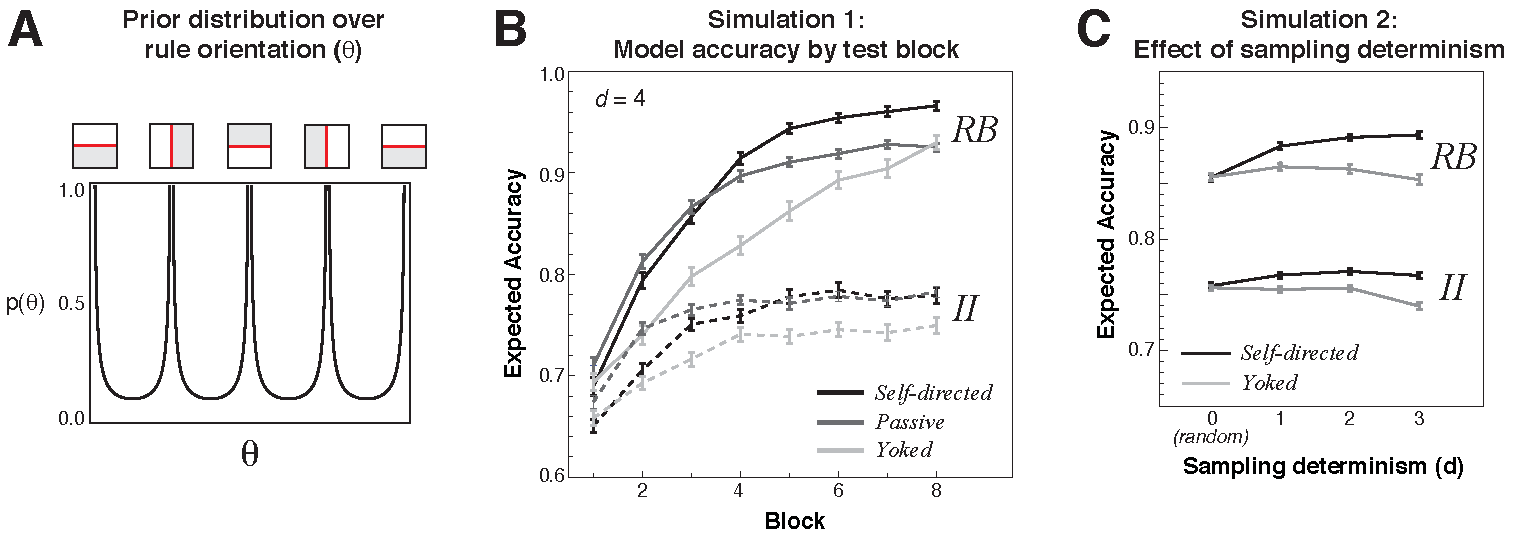
\includegraphics[height=2.5in]{figures/simresults_rev.pdf}}
\caption{\textbf{A:} Distribution defining prior bias for axis-aligned (uni-dimensional) rules. \textbf{B:} Simulation 1 results. Expected accuracy of models in each training condition qualitatively match the behavioral performance shown in Figure~\ref{accuracy.fig}B. \textbf{C:} In Simulation 2, models were trained over a range of values of sampling determinism; as $d$ increases, the average distance of samples from the self-directed model's hypothesized category boundary decreases. Increasing values of $d$ led to higher expected accuracy for the self-directed model, while there was no change in the expected accuracy of yoked models trained on the same data (similar to regression lines in Figure~4A).}
\label{simresults.fig}
\end{figure*}


\subsection{Simulation 1: Classification performance}

Our first goal was to evaluate whether the model could capture the overall pattern of results found in our experiment. Five-hundred runs of self-directed, passive-normal, and passive-yoked models were trained in both RB and II tasks.   Self-directed models generated new observations on each trial (using Equation~\ref{labelentropy.eq} and~\ref{choiceprob.eq}), but were otherwise identical to passive models, with the exact same parameter settings shared across all three groups and for both the RB and II tasks.  Table~\ref{par.fig} describes the full set of parameters in the model along with the settings used in our simulations (parameters were optimized by hand to the pattern of overall classification accuracy).  For each run of the self-directed model, a paired passive-yoked model was given the same exact sequence of training examples. Passive-normal models were trained using data generated from the same distributions that were used in the behavioral experiment. For all training conditions, the model was tested on the same test items from the experiment, presented in a randomized order. 

Using a single set of parameters across conditions, the results of the simulation (Figure~\ref{simresults.fig}B) closely match the overall accuracy from the behavioral results. First,  accuracy was greater in the RB task than the II task in all conditions. This effect is dependent on two main assumptions in the model: a prior bias toward uni-dimensional rules, and a small memory for recent observations ($n=5$). In the RB task, learners quickly converge on the right form of uni-dimensional rule, and over the course of learning refine its exact location (by adjusting the bias term). In the II task, however, the small number of stored observations is not enough evidence to consistently overcome the prior bias. Thus, throughout learning the active hypothesis alternates between modes of the posterior corresponding to axis-orthogonal rules. As in our behavioral results, the model can successfully acquire the correct II rule, but it is less likely to maintain that hypothesis over time. 

Second, the self-directed model performed better than the passive-normal model in the RB task. As predicted, this occurs because the self-directed model is able to generate samples close to the true category boundary, while the passive-normal model is limited by the distribution of training samples. Inspection of the sequence of hypotheses generated by the model showed that the passive-normal model had higher variability in the bias term during learning, showing that the training data was less effective at maintaining a hypothesis in the center of the stimulus space. Notably, the difference between conditions does not occur in the II task, in which the model is biased against adopting the correct form of rule in either training condition.

\begin{figure*}[t]
\centerline{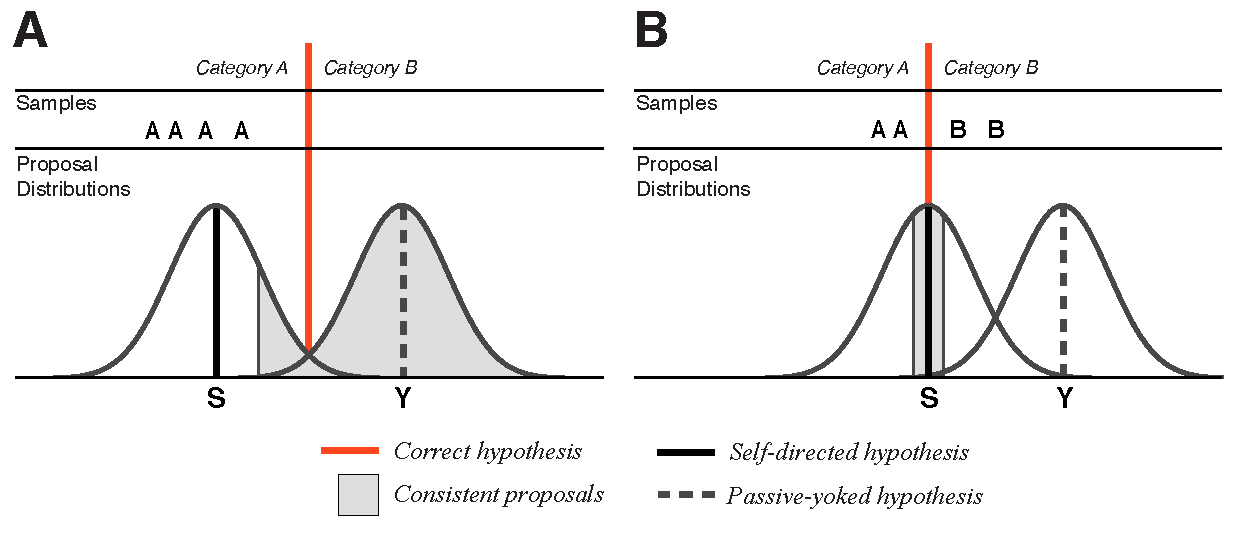
\includegraphics[height=2.5in]{figures/search.pdf}}
\caption{Interaction of observations and hypothesis generation for a uni-dimensional hypothesis set (see description in text).
}
\label{model.fig}
\end{figure*} 


Finally, the simulation captures the divergence between self-directed and passive-yoked learners in both RB and II tasks, despite sharing the same training data and identical parameter settings. This divergence arises directly from the model's stochastic process of generating new hypotheses during learning, such that a single observation may differ in how it influences the acceptance of a new hypothesis. 

To provide a more concrete intuition for why self-directed and passive-yoked learners diverge in this simulation, a simple illustration is given in Figure~\ref{model.fig} (using a univariate categorization task for simplicity).  The horizontal axis of the figure corresponds to the single continuous feature dimension (e.g., size), and the set of potential hypotheses is any criterion on that dimension such at any stimulus to the left of the criterion is in category `A' and anything to the right is in category `B'. The true category boundary is shown by the red line, while the currently active hypothesis of the self-directed learner is shown with a solid black line, and the active hypothesis of the passive-yoked learner is shown with a dashed line. The Gaussian proposal distributions depict the likelihood of new hypotheses being generated (centered on the current hypothesis). In panel A, both learners have an incorrect hypothesis about the category boundary. The self-directed learner selects samples close to its active hypothesis (shown by the location of ``A" observations along the top of the figure), which then limit the set of potential proposals that may be adopted to replace the active hypothesis (gray region under proposal distributions). Such proposals will tend to move the self-directed learner in the direction of the correct rule. In contrast, almost all proposals that may be generated by the yoked learner are equally acceptable given the recent set of observations. As a result, the yoked participant will adopt a proposed hypothesis even if it is more distant from the correct rule. In panel B of Figure~\ref{model.fig}, the active hypothesis of the self-directed learner is correct, while the passive-yoked learner is incorrect. Observations selected by the self-directed learner limit changes to its current hypothesis. While the same observations provide disconfirmatory evidence for the yoked model, the likelihood of generating a proposal consistent with that data is very small (gray region in the tail of the proposal distribution). As a result, the ability of the passive-yoked learner to discover the correct rule will depend on a extended stochastic search process, which will tend to result in poorer performance.

The key point of this simulation is that interactions between the learner's current hypothesis, the hypothesis generation process, and the self-directed sampling strategy can influence learning outcomes. Learners who differ only in whether they control the selection of new observations can diverge in performance, even if they have had the same training experience.

%This divergence arises due to the model's stochastic process of generating new hypotheses during learning. Deterministic sampling, while providing evidence that may disconfirm an incorrect hypothesis, also limits the set of proposals that are acceptable. The ability of a yoked model to generate proposals from that set is limited by the search process itself (i.e., the distance from the current hypothesis, how proposals are generated, etc.). 

\subsection{Simulation 2: Explaining the systematic divergence in self-directed/yoked performance}

While Simulation 1 captures the overall effects of training condition and category structure, we were additionally interested in explaining the systematic divergence in performance between self-directed and yoked participants as it related to sampling behavior. Note that in Figure~\ref{scatterplots.fig}, performance among self-directed learners is correlated with how effective the participants were at sampling. Subjects who sampled closer to the true boundary (and their own subjective boundary) performed better at the categorization task.

%\hl{While Simulation 1 captures the overall effect of conditions, we were additionally interested in explaining the systematic divergence in performance
%between the self-directed and yoked participants.  Note that in Figure}~\ref{scatterplots.fig}\hl{, there is a wide range of performance amongst self directed learners
%and this range in performance is correlated with how effective the participants were at sampling.  In particular, subjects who sampled closer
%to the true boundary (and their own subjective boundary) performed better at the categorization task.}

%Given that we found a strong relationship between sampling ability and accuracy in our experiment, we werespecifically interested in how the randomness of sampling behavior (controlled by the determinism parameter $d$) would affect overall performance for both self-directed and passive-yoked models. Thus, we ran simulations for a range of values of $d$ and compared the overall accuracy between simulations (all other parameter values were the same as in Simulation 1). 
In order to explain these individual differences, we explored the
impact of the sampling determinism parameter ($d$) on learning.
Recall that the $d$ parameter governs the degree to which the model ``exploits" its current uncertainty.
In our simulation, we ran a new set of self-directed simulations with a range
of values of $d$.  We then presented the data sequences generated from these simulations to a set of yoked models which used the
same parameter settings.  The results are presented in  Figure~\ref{simresults.fig}C. 

When $d=0$, new samples are generated randomly from the stimulus space, and performance is equal for both self-directed and yoked groups. As $d$ increases, however, new samples are increasingly likely to be close to the self-directed learner's hypothesis. Consistent with our finding of a strong relationship between sample distance and accuracy (Figure~\ref{scatterplots.fig}), the increase in determinism improves performance for the self-directed model (particularly in the RB task). The same change in the distribution of samples does not improve passive-yoked performance, and even leads to a decrease in overall accuracy at higher values (since it becomes increasingly difficult to generate a hypothesis consistent with samples that are extremely close to a decision bound). 

While this simulation is a simplification of the sampling behavior seen in our experiment (e.g., sampling may have varied in determinism over time), it provides a mechanistic explanation of how sampling influences the speed of learning. 
In general terms, it suggests that the opportunity to sample information is not necessarily enough to improve performance. Instead, the ability to sample data that tests one's current hypothesis (as opposed to a random observation) is central to the benefit of self-directed learning.

%While this simulation is a simplification of the sampling behavior seen in our experiment (e.g., sampling likely varied in determinism over time and between participants), it provides a mechanism by which both the ability to sample information, and the quality of the samples generated 


%Finally, the stochastic nature of learning in the model---characterized by local, probabilistic adjustments to the current hypothesis---allows the quality of sampling to influence the speed of learning. In our simulation, expected accuracy increased as the value of sampling determinism increased . While this is a simplification of the sampling behavior in our experiment (e.g., sampling varied in determinism over time and between participants), it provides a potential account of the relationship between sampling ability and performance for self-directed learners. Generally, samples that are more deterministic (close to the hypothesized category boundary) provide diagnostic evidence for the self-directed learner. If their hypothesis is correct, samples close to the boundary make it highly unlikely that proposed changes to the hypothesis will be accepted. If their hypothesis is incorrect (e.g., a uni-dimensional rule on the wrong dimension), the samples strongly disconfirm the current belief and encourage shifts to a different type of hypothesis.


In conclusion, while the processes of hypothesis generation and sampling are idealized in the model, the simulated results are remarkably consistent with the pattern of behavioral results. The model details a process through which a divergence between self-directed and passive-yoked performance may emerge, while incorporating common assumptions from existing category learning theories (e.g., a preference for unidimensional rules, probabilistic decision boundaries). In addition, our basic framework follows directly from Bayesian learning principles, but incorporates realistic constraints about how people search through the space of hypotheses and remember prior examples. It is important to note that these capacity constraints are critical for achieving the behavior of the model. Increasing either the number of hypotheses maintained or the number of observations stored in memory will tend to lessen the influence of sampling decisions.  Thus, only through the interaction between the
various components of the model do we gain insight into the advantage of self-directed learning.

%While the processes of hypotheses generation and sampling are idealized in the model, the simulated results are remarkably consistent with the pattern of behavioral results. The model provides a process through which a divergence between active and passive-yoked performance may emerge, while incorporating common assumptions in previous accounts (e.g., a preference for unidimensional rules, probabilistic decision boundaries).  Our basic modeling framework follows directly from Bayesian learning principles, but incorporates realistic, process-level constraints about how people search through the space of hypotheses about the category. It is imp


%Importantly, our simulations suggests that effective sampling may not simply be a byproduct of successful learning, but rather that it allows people to bootstrap their own ability to acquire (and maintain) concepts more efficiently. 


%One way that the model can account for differences between active and passive-yoked groups is by assuming that active participants represent more than one hypothesis at any given time (consistent with the generalized ``engagement" hypothesis described in the Introduction). In the model, this might correspond to an increase in the number of point estimates of the posterior maintained in working memory. To evaluate this idea, active participants were modeled using a set of 5 posterior samples per run (in contrast to one sample used for the passive groups), with the additional assumption that learners classify items according to the most likely hypothesis from the set they are considering. As seen in Figure~\ref{model.fig}A, the greater number of samples leads to higher accuracy over the passive groups in the RB task, but not in the II task. While a change in the number of particles maintain considered is consistent with the idea that active learners are more cognitively engaged in the task (and thus search the hypothesis space more effectively), further work is needed to directly test this representational hypothesis. At the very least, the potential divergence between the sequence of data observed in the task and the sequence of hypotheses considered by the learner provide a potential mechanism for explaining the active/passive-yoked distinction.

%Finally, we were interested if samples generated by the active models show the same pattern as produced by our participants. Simulated samples were generated using \emph{margin sampling}, in which an observation is most likely to occur when its predicted likelihood of belonging to category A and B are equal (i.e., the likelihood of making an observation $o^t$ was proportional to $1-|P(o^t=A|  \textbf{w}, b, \sigma)-P(o^t=B|  \textbf{w}, b, \sigma)|$).  As seen in Figure~\ref{model.fig}B, the predict sampling distribution qualitatively matches the behavioral results. In the first block of both tasks, the model produces samples that are widely dispersed throughout the feature space. By the final block, RB models have converged on the true boundary, querying the margin of the boundary where uncertainty is greatest. In the II task, the diffuse distribution of samples reflects the variability in the hypotheses under consideration.

\section{General Discussion}
In their landmark work on concept acquisition, \citet{Bruner:1956p13030} discuss the distinction between learning through \textit{selection}---a self-directed information sampling strategy---and learning through \textit{reception} --- a passive mode in which the learner must ``make sense of what happens to come along, to find the significant groupings in the flow of events to which he is exposed and over which has only partial control" \citep[][p.126]{Bruner:1956p13030}. Subsequent theories of category learning have focused almost exclusively on the latter type of learning, with the typical experimental approach ensuring that all participants experience the same distribution of items from each category. One consequence of this focus is that existing models fail to account for how people might make sampling decisions during category learning or how these decisions might influence patterns of acquisition~\citep{Gigerenzer:2006lt}.  This strongly limits the generalizability of these theories relative to the range of strategies people use during natural concept learning~\citep{markman2003category}.  Our work in this paper was aimed at revisting this somewhat overlooked learning mode distinction in the context of a well-studied perceptual classification task.

% In addition, this focus on a particular kind of learning task runs the risk of underestimating how quickly people can learn when they have more control over their learning experiences (as demonstrated in our RB task). 

\subsection{Adaptive sampling: selecting data that is best for you (and only you)}

Previous research has often attributed a self-directed learning advantage to being more mentally ``active" or ``engaged"~\citep{bruner1961act}, or focused on differing assumptions made by learners depending on their role in collecting data. In contrast, we have proposed that the advantage is a natural consequence of a stochastic, sequential hypothesis testing process. First, when the true category structure is consistent with their prior biases, self-directed learners can adaptively collect information that is more useful than a typical dataset specified by the experimenter. Second, the asymmetry in learning outcomes associated with self-directed and yoked learners derives directly from the mechanistic way in which participants search the space of hypotheses during learning, and the simple fact that self-directed learners can choose data to test their specific beliefs while the yoked learner cannot. Critically, our account assumes identical hypothesis spaces, learning strategies, parameters, and priors for all groups. In this sense it makes a strong appeal to mechanistic process models which articulate in more detail the representations and stages of information processing that guide learning~\citep{Sakamoto:2008ay}.  

An important inspiration for the present study is recent machine learning research showing that allowing artificial learners to sample information about which they are uncertain can improve learning efficiency in a broad range of real-world problems~\citep{Castro:2008p12850,Cohn:1992tw,Dasgupta:2005xv,Mackay:1992kn,Settles:2009p13423}.  The motivation behind this research is that in many real-world situations explicit instruction and feedback is sparse and expensive (e.g., obtaining human judgements about the content of online videos).   In these cases, it is advantageous for a machine learning algorithm to make intelligent decisions about which information is expected to be useful and request labels or feedback for only those items (typically, those for which the classifier is currently most uncertain).   This technique has been used to develop ``curious" machine learners that can perform well with less explicit training~\citep[c.f.][]{schmidhuber1991curious,Murphy:2001rp,Tong:2001if,Cohn:1992tw}.

Our results show that achieving similar improvements in efficiency in human learners depends on the structure of the concept being learned. For example, in our II task there was no benefit for self-directed learning over passive, observational training.  The explanation that we advanced in our modeling simulations is that learners approach such tasks with a strong prior bias toward simple, uni-dimensional rules~\citep{Ashby:1999ig,Ashby:2002p13331,Gureckis:2002ys} which ultimately leads to lower overall performance in the II task, regardless of the learner's ability to design samples.   
%Another possibility is that self-directed sampling requires a form of explicit reasoning that is incompatible with the type 
%of implicit, procedural memory that has been proposed to underlie II learning~\citep{Ashby:1998p8468}.  By this later account, self-directed learning might even encourage a perseverative search for simple rules could lead to an overall \textit{disadvantage} in relation to passive learners given more extensive II training.  (Note that in our study, there was a slight ordinal advantage for the passive-normal group over the self-directed group in the II task.)

\subsection{How do people make information sampling decisions?}

As shown in Figure~\ref{sampledistance.fig}, our self-directed learning procedure provides a rich source of
data about how people search for information while learning.  Perhaps the most  striking pattern was that participants in the RB task concentrated their samples near the true category boundary in the later part of the task.  Of course, one possible explanation is that self-directed learners' ability to sample in this region simply reflects learning that has already occurred. This seems unlikely, however, given that participants continue to sample near the category boundary even after achieving high performance (in the RB task) and despite the added effort required to design samples. 
%This suggests that people continue to rely on samples along the category boundary to maintain and refine their beliefs.   

The question of how humans 
make intuitive judgments about the ``usefulness" of new observations has been the focus of extensive study in the hypothesis testing 
literature~\citep{Wason:1960gf,Skov:1986jw,Klayman:1987os,Oaksford:1994tw,Ginzberg:1996bh}.  
Early findings raised concerns about the human ability to identify the value of future information (e.g., the pervasive evidence of confirmation bias, Wason, 1960; see Nickerson, 1998 for a review).   Our study provides a
counter-example to this well known effect in that participants quite effectively sought discriminating information about the
categories in the RB task. In our simulations, we assumed that learners adopted a ``rational" information selection strategy by favoring items which they were least certain (i.e., those close to the category margin).   However, at this point, our sampling data do not appear to uniquely support any particular model of sampling decisions (e.g., impact, information gain, and KL-divergence all make somewhat similar predictions in the current task, Nelson, 2005).  

%one hypothesis for this difference between tasks is that the ability to effectively design samples requires a kind of meta-cognitive access to the current hypothesis which is unavailable to II learners (consistent with the implicit/procedural learning hypothesis in COVIS,~\citet{Ashby:1999ig}). A more straightforward 

It is interesting that participants in the II task were generally unable to sample as effectively as RB participants. It is undoubtedly more difficult to design samples that fall along the diagonal since it requires specifying values along both stimulus dimensions. Notwithstanding the increased effort required, one explanation might be that participants in the II task \textit{are} in fact sampling effectively (i.e., in regions of the space for which they are most uncertain). However, this uncertainty is evaluated \textit{with respect} to the limited set of hypotheses the learner is actually considering at any point in time~\citep{Bonawitz:2010fk}. Consistent with the above discussion, our decision-bound analyses suggested that learners in the II task persisted in using simple, uni-dimensional rules throughout the task. Thus, the pattern of diffuse sampling in the II task may reflect optimal sampling along a sub-optimal and frequently shifting uni-dimensional boundary. Since II learners in our task never achieved the same high performance as RB participants, we were unable to test whether the same convergence on the true decision boundary might occur. However, examination of individual II subjects revealed a few participants who were actually quite effective at sampling along the diagonal boundary, and these participants were among the highest performers in their group. 

Of course, our theory is necessarily simplified, and the actual pattern of sampling data observed in our study might reflect 
a mixture of multiple processes and strategies. For example, self-directed sampling may serve an adaptive memory function by allowing participants to ``remind" themselves of past experiences which been individually forgotten.  Indeed, certain instances of what might look like ``confirmation bias" in our task may simply be participants' attempt to remind themselves about particular regions of the stimulus space and to verify that the task structure hasn't changed.  Subject to such cognitive constraints, Figure~\ref{model.fig}B points outs out how effective sampling can also help participants to hold the correct hypothesis in mind.
%=======
%Of course, the actual pattern of sampling observed in our study might reflect multiple processes and strategies. Thus far we have examined the use of self-directed sampling to avoid redundant data and disambiguate competing hypotheses, which has also tended to be the focus of previous research on hypothesis testing~\citep{Oaksford:1994tw,Nelson:2005ph,Kruschke:2008ph}. However, our results highlight an additional function of self-directed sampling in allowing participants to ``remind" themselves of past experiences which have been forgotten. 
%Indeed, certain instances of what might look like ``confirmation bias" in our task may simply be participants' attempt to remind themselves about particular regions of the stimulus space and to verify that the task structure hasn't changed. Furthermore, our simulations assumed that learners consider only a single hypothesis at a time and evaluate that hypothesis with respect to only a subset of the most recent observations.  Subject to such cognitive constraints, effective sampling not only reveals information about potential hypotheses, but also helps participants to hold the correct hypothesis in mind.
%>>>>>>> .r1084


%Of course, the actual pattern of sampling data observed in our study might reflect 
%multiple processes and strategies. Thus far we have focused on the use of self-directed sampling to avoid redundant data and focus on regions that are most informative. 
%Self-directed sampling may also serve an adaptive memory function by letting participants ``remind" themselves of past experiences which have been forgotten. Interestingly, research on hypothesis testing strategies have tended to focus primarily on the role of information sampling in disambiguating competing hypotheses~\citep{Oaksford:1994tw,Nelson:2005ph,Kruschke:2008ph}. However, the importance of memory constraints in our simulations suggest   However, our simulations also highlight this possible secondary role. 

%This 
%dynamic interaction between information search and learning/memory processes offers a somewhat novel 
%take on classic issues of hypothesis testing behavior.

%On the other hand, information search behavior in other tasks (such as planning  saccades) has been shown to be close to optimal~\citep{Najemnik:2005ph}, and research on
%how people use interventions to learn about causal structure have often shown the effectiveness
%of active learning strategies (Steyvers et al., 2003; Lagnado \& Sloman, 2004; Sobel \& Kushnir, 2006).  
%Even young children show evidence of directed, uncertainty-driven exploration by playing more with a toy after seeing confounded evidence about how it works~\citep{Schulz:2007rf}. 


% theoretical points:

% sample - adds to people's memory
% sampling might increase engagement
% sampling improves subject's ability to select better data
% research on hypothesis testing tend to emphsize issues primarly concerned with the third point, and debates
% about if people exhibit 
% our results suggest a slightly different perspective in that active sampling should be viewed as a part of the learning
% process itself

% learning models - inference, classification, etc...  trial order effects


\subsection{Different learning outcomes from the same data: A challenge for existing models}

One of the most interesting findings was that yoked subjects who saw the exact same observations  performed worse than their self-directed counterparts.  This suggests important differences between self-directed and passive learning that are difficult to explain using existing models. In fact, our results are essentially incompatible with most models of category learning which assume that learners update their beliefs through a common process~\citep{Nosofsky:1984cl,Kruschke-1992um,Love-2004bp}.  Even assuming individual differences in initial weights in a model such as ALCOVE or SUSTAIN would not lead to a systematic performance
deficit for yoked participants.  

%In addition, these results appear to violate the \textit{likelihood principle}, a central tenant of  Bayesian inference.  According to the likelihood principle, inferences should depend only on the likelihood of the actual data received~\citep{Mackay:1992kn}.  

Similarly, these results are problematic for any model in which both the self-directed and passive-yoked learners optimally update their beliefs based on observed data alone.  In order to accommodate the self-directed/yoked divergence in a Bayesian framework, one must assume that learners apply either a different likelihood function depending on the learning mode, or a different prior\footnote{Perhaps a third way that a completely Bayesian model could account for these results would be to assume that self-directed and passive-yoked participants integrate evidence from a different subset of the training data.  However, given the additional task demands of designing individual stimuli on every trial, it would be most reasonable to assume that self-directed participants would be more limited in this regard. Instead, the less distracted yoked participants systematically under-performed their self-directed counterparts.}. 
Intuitively, it is unclear why a learner would make a different prior assumption about possible category structures depending on self-directed or passive learning since the structure of categories in the world are independent of the manner in which information is collected. On the other hand, some recent work has argued that human learners adopt different likelihood
functions depending on assumptions about the process which generated 
observations~\citep{Tenenbaum:1999ao,Tenenbaum:2001wq}. According to ``weak sampling" the learner assumes the examples are chosen independently of the true concept.  In contrast, ``strong sampling" assumes that the generating process itself is informative about the underlying concept.  Self-directed information sampling justifies a ``weak sampling" assumption since the learner should correctly recognize that their own information collection decisions are independent of the target concept (since they don't yet know it).  In contrast, strong sampling is justified in pedagogical settings where learners are  instructed by a knowledgeable teacher~\citep{Xu:2007rt,Xu:2007yq,Shafto:2008p6011,Gweon:2010nx}.

However, it is less clear that such distinctions
are useful for explaining behavior in discriminative classification tasks.  In most of the work on strong versus
weak sampling the emphasis is on learning generative models from positive examples alone \citep[c.f.][]{Tenenbaum:1999ao,Tenenbaum:2001wq,Xu:2007rt}.
Under both strong and weak sampling assumptions, the location of a linear decision boundary can be
quite accurately specified using only a few examples, particularly when those examples fall close
to the true category boundary.  However, as shown in our results, self-directed learners and
yoked learners have quite different learning patterns despite receiving equally constraining data. This was particularly striking in the RB task, in which the data provided to yoked learners tended to be highly informative about the correct boundary. In addition, we found no difference in accuracy between passive-yoked learners whether or not they were aware of the source of their training data, suggesting that such prior knowledge did not play a significant role.

Instead, our theory assumes that self-directed learning increases the congruence between the current hypothesis under consideration and the actively gathered data.  Our simple model based on this principal is able to explain the diverging
pattern of inference in the self-directed and yoked groups with a single set of shared parameters and learning mechanisms.

%For example, people are willing to make stronger inferences based on data that is generated by a teacher than when generated randomly~\citep{Shafto:2008p6011}. In our study, 




\subsection{Relation to other theories of category learning and sequential hypothesis testing}

%Aside from the fact that existing models make few predictions about sampling behavior, our results highlight a more specific challenge for any model that assumes equivalent learning given identical training sets. Our model accounts for the divergence between active and yoked learners through the interaction of simple assumptions that closely follow from 
The modeling framework that we propose bears a strong resemblance to existing work on sequential hypothesis testing~\citep{Bower:1964kn,gregg1967process,millward1973direct,thomas2008diagnostic,nosofsky1998rule}. According to these models, learners maintain a restricted set of distinct hypotheses at any given point during learning, and use new observations to eliminate entries in that set. The makeup of the current set of hypotheses influences how one evaluates data and generates new hypotheses~\citep{thomas2008diagnostic}. Differences between individuals (e.g., due to random initial hypotheses or differences in memory capacity) can lead to divergent hypothesis sets, even if they are exposed to the same evidence.

It is interesting to consider the relationship between these classic models and recent work on ``process-level" approximations to fully Bayesian models of cognition~\citep{brown2009detecting,Ullman:2010p14180}. Like the model we have presented, these theories assume that the learner selects a subset of hypotheses to consider based on a stochastic process such as MCMC sampling.  There are a number of attractive features of this approach that go beyond older work on serial hypothesis testing. First, so called ``rational process models" allow one to specify a prior over hypotheses, which is particularly useful when that prior is for an abstract property of many hypotheses (e.g., a preference for simple rules on any one dimension). Second, because the models are approximations to a fully Bayesian solution, they allow characterization of suboptimalities in people's behavior~\citep{brown2009detecting}. Understanding how people diverge from an optimal solution may help to narrow the range of potential process models that are appropriate.

Finally, it should be noted that existing models of category learning have attempted to incorporate some aspects of rule learning, and are in many ways consistent with the model of sequential hypothesis testing we propose. For example, RULEX \citep{nosofsky1998rule} assumes a stochastic process of rule generation and a preference for simple unidimensional rules, while allowing for encoding of individual exceptions to the hypothesized rule. COVIS~\citep{Ashby:2010p14184} proposes that a rule-learning system represents a set of potential rules (generally single-dimensional, or conjunctive/disjunctive rules on two dimensions). Some rules may have greater ``salience" than others if they are \textit{a priori} more likely (e.g., single dimensional rules begin with greater salience than conjunctive or disjunctive rules), and the salience of an adopted rule is adjusted up or down based on whether it is consistent with subsequent observations. %The generation of new rules is then a simple probabilistic function of this salience measure. 
Rather than starting from scratch,  our approach incorporates many of the same principles evident in existing theories of learning.  However, our contribution focuses on how these principals interact with self-directed sampling to determine learning outcomes.

%\subsection{Selection strategies}



%\subsection{Implications for other tasks}
%
%Learning in dynamic environments often involves information generated by a range of sources. This may include samples provided by other people with different backgrounds or goals (e.g., educators that are motivated to teach a concept). As such, learning requires coordination of internal hypotheses with knowledge about the source of the observed data. For example, people are willing to make stronger inferences based on data that is generated by a teacher than when generated randomly~\citep{Shafto:2008p6011}. In our study, we found no difference between passive-yoked learners whether or not they were aware of the source of their training data.

%\subsubsection{Relationship to existing models}
%\subsection{Relation to previous work}

%For example, Fazio, Eiser, and Shook (2004) who studied 
%the impact of experiential sampling on category acquisition.  Participants in their study were 
%presented with ``beans" that varied along two  continuous dimensions and were asked on each 
%trial if they would like to (virtually) eat the 
%bean and find out if it was healthy or poisonous.  Decisions to not eat a particular bean 
%thus provided no information (i.e., feedback in the task was contingent on sampling decisions,
%see the description of \emph{selective sampling} below). 
%Experiential learners were found to be risk averse, in that they showed a bias to think that 
%novel beans were bad.  In addition, participants were more accurate classifying bad beans 
%than good beans.  This asymmetry in learning only occurred in situations where learners 
%made the sampling decisions themselves: if full information was provided on each trial 
%irrespective of the decision to ``eat" a bean, participants showed 
%equal classification performance for both categories.   
%However, outside of these studies (and a few directed at understanding how people use interventions to
%differentiate between different causal structures~\citep{Steyvers:2003ee}), less work has examined 
%the impact of active sampling/active learning in category and concept acquisition and this work has 
%yet to have an significant impact on models of category and concept acquisition.


%
%It is important to note that the Active training in our experiment represents an extreme mode of selection, in which the learner is forced to choose a new training item on every trial. It is likely that in real-world situations people shift between modes of learning. For example, people may prefer to begin learning by passively observing a number of exemplars in order to construct a representation of the categories~\citep{avrahami1997teaching}.

% For example, Atkinson (1972a, 1972b)
%examined the ability of participants to learn novel English-German vocabulary pairs with the
%goal of developing individualized optimal training procedures.  Word pairs were assumed to be
%in one of three states: unknown, permanently known, or in between (i.e., on the threshold of transitioning
%to being permanently stored).
%In a baseline condition, participants were given a random word pair to study on any given trial.
%In a second condition, participants were allowed to select which items to study at any point (i.e., active 
%learning).  In a final condition, a computer-based training procedure was used that presented items that were
%estimated to be most likely to be at the threshold of ``permanently" learned.   Participants in the
%active learning condition performed 53\% better than those in the random control condition, while
%participants in the computer aided condition gained 108\% over the control, suggesting that participants
%can use their current state of knowledge to guide learning (but that it is possible to improve even
%further with external support, see also \citep{Nelson:1994qa,Kornell:2006fu}).  \citep{sobel2006importance}


\section{Conclusions} 
%(cf.,~\citep{Chin-Parker:2010uq})

Self-directed information sampling may be a common way for people to learn about categories 
in the real world, but it has been rarely studied in experimental contexts. Our results join a growing number of studies in demonstrating that learners can effectively bootstrap their own learning through self-directed exploration of their environment~\citep{Atkinson:1972rz,Atkinson:1972rm,Fazio:2004jw,Castro:2008p12850,Steyvers:2003p5901,sobel2006importance}.
Importantly, our results show that this facilitation is dependent on the structure of the learning problem. 
We found that self-directed learners were able to make informative queries to support their learning, but were more successful at doing this for RB categories than II categories. In addition, self-directed learners systematically out-performed participants who were yoked to their observations.  Our simulations explain these results through the interaction of a capacity-limited hypothesis search process, a bias toward  uni-dimensional rules and a limited memory for recent observations. To the degree that participants prefer particular types of rules, their sampling behavior will tend to be sub-optimal when the target rule mismatches these expectations, a similar point made in analyses of active machine learning~\citep{Mackay:1992kn,Settles:2009p13423}. As such, our results may have important implications for the settings in which self-directed learning can be more effective than passive, teacher-led instruction. 

%In this framework, sampling plays a central role in allowing a learner to discover the correct category 
%boundary. When the person can sample effectively, they may be able to adaptively mold their training experience to focus on 
%data that is useful with respect to their particular set of beliefs. 

%In our experiment, active learners were able to make informative queries to
%support their own learning, but this ability was more successful for RB categories than for II categories. 
%Our simulation results explain this difference in terms of a bias toward considering rules along
%a single dimension.  In addition, we evaluated one explanation for the divergence between active
%and passive-yoked participants, namely that active participants consider a greater number of hypotheses
%about the latent category structure.  

%Our general  finding that the effectiveness of active sampling may depend on the structure of the category adds to recent work examining active learning in binary classification tasks~\citep{Castro:2008gd}.  While a number of theorists have attempted to explain active data selection in terms of optimal information gain~\citep{Oaksford:1994tw,Nelson:2005ph}, our results  suggest that the ability to design useful queries is strongly limited by the hypothesis search process that guides learning.  
%To the degree that participants prefer particular types of rules, their sampling behavior will tend to be sub-optimal when the target rule mismatches these expectations, a similar point made in analyses of active machine learning~\citep{Mackay:1992kn,Settles:2009p13423}. In summary, active learning may promote learning, but it works best when you have a strong and correct idea of what you are trying to learn.

%
%The results of the present study demonstrate a clear advantage for active learning in a well-understood category learning problem. Moreover, we have shown that the improvement for active learners cannot be accounted for solely by the statistical information in their queries, as shown by the poorer performance of passive-yoked participants. While future work will investigate in greater depth the processes that contribute to this effect, we have offered one potential explanation: by considering multiple hypotheses during learning and leveraging their uncertainty to select new observations, active learners converge on the correct solution more efficiently. 
%
%Our preliminary modeling of the results in this task offers a potential mechanism to explore in order to understand why active participants perform better than their passive-yoked counterparts. While increased engagement in a learning problem has often been cited in support of active inquiry learning (e.g., in pedagogical contexts, cf. Bruner, 1961), the present study is an attempt to understand the cognitive components of that engagement.


%
%Procedure for test blocks differed from previous studies by using a uniform grid of test items over the entire space, rather than additional samples from the category distributions. 
%Psychologists and educators have long recognized that human learning is, at least in part, an active 
%processes involving the search for new information that enriches our understanding of the 
%world and reduces our current uncertainty (cf. ~\citep{Piaget:1930hp,Bruner:1961vn}).
% In the domain of casual learning, researchers have shown 
%that the ability to interact with a causal system through active interventions can, in many cases,
%improve learning of the causal structure between a set of variables~\citep{Steyvers:2003ee,Lagnado:2004hs,Sobel:2006gf,Schulz:2007jt}.  In addition, Sobel \& Kushnir (2006) showed that the advantages for intervention-based
%learning may depend on the active engagement of the learner in designing interventions (passive controls 
%who were yoked to intervention learners did not show the same
%learning benefits).  In the domain of category learning, Castro, et al. (2008) 
%found that allowing learners to  actively select training examples improved the efficiency 
%by which they learned a linear decision boundary in a uni-dimensional concept learning task 
%(see also \citep{Fazio:2004jw,Gureckis:2009hm}).   However, across these studies there has been
%little theoretical analysis to explain exactly why active/intervention based learning might
%improve learning, the mechanisms that might underly how people design particular intervention,
%and the limits of this kind of learning.
%However, both the distribution and sequencing of exemplars in category learning tasks
%has been shown to strongly influence learning~\citep{Elio:1984zn,Medin:1994nb,Mathy:2009hc}.  Given this, one natural
% question concerns the impact that letting learners query items they would like to know more about might
% have on the learning process.

%
%In the present paper, a growing number of papers have demonstrated that, relative to random (passive) sampling, active learning can improve the ``sample efficiency" of learning complex concepts (i.e., number of training exposures needed to reach a particular threshold 
%of classification error)~\citep{Cohn:1992tw,Mackay:1992kn,Dasgupta:2005xv,Castro:2008gd,Settles:2009kk}.  
%For instance, ~\citep{Dasgupta:2005xv} proved that actively querying points near the current 
%margin of a simple linear classifier can result 
%in an exponential decrease in the number of training episodes needed to reach a given level of error.  
%Much of the research effort in this area is focused on designing information sampling norms or 
%metrics which assign value to future observations based on the potential for information.
%One of the key contributions of the current proposal is to evaluate some of these metrics as proposals
%for how humans might sample information during learning.

%

%\begin{figure}[t]
%\centerline{\includegraphics[height=1.5in]{figures/II_overall_acc.pdf}}
%\caption{\small{Overall accuracy over training blocks. Active (), Passive (), Yoked().}}
%\label{II_acc.fig}
%\end{figure}


%\small{
%\subsubsection{Acknowledgements}
%We would like to thank Louis Tur for programming assistance.
%}


%Note that a number of models have been proposed for how people classify items with 
%continuously-valued features using simple rules~\citep{nosofsky1998rule,Ashby:1998p8468}. 
%However, there have been fewer formulations of an inference procedure that describes how these
%rules are generated of change during learning.  One prominent counter example 
%is COVIS~\citep{Ashby:1998p8468}, in which an explicit rule-generating system competes with an 
%implicit exemplar-based system to produce responses. Importantly, people are assumed to rely 
%initially on the explicit system, with a strong bias toward using uni-dimensional rules for classification. 
%One source of evidence for this competition is behavior in the II task, in which early responses are best 
%fit by suboptimal, uni-dimensional decision boundaries, and learning of the correct II boundary emerges 
%slowly over the course of training~\citep{maddox2004dissociating}. Given the relatively small amount of training data and the use of observational training in our II task, our results likely reflect an early stage of learning in which participants attempt to use uni-dimensional rules~\citep{Ashby:2002p13331}. While there are many examples of this preference for simple rules during classification, there have been relatively few formulations of an inference procedure that describes how these rules are generated and change during training (however, see~\citep{erickson1998rules,Ashby:2010p14184}). As suggested by our preceding analyses, however, a model of this process is critical for understanding why active and passive-yoked learners achieve different performance given identical training sets. As such, it is unclear how existing models might account for this divergence, as well as the relationship between sampling patterns and accuracy. 





%\section{Appendix A: }
%
%\begin{table}[t] \caption{\small Comparisons of variability of best-fit parameters between training conditions for both early and late blocks using Wilcoxon rank sum test.}
%\centering
%\begin{tabular}{ | c | c | l l | l l | l l | l l | } \hline
%& & \multicolumn{4}{c|}{RB} & \multicolumn{4}{c|}{II} \\ \hline
%& & \multicolumn{2}{c|}{Early} & \multicolumn{2}{c|}{Late} & \multicolumn{2}{c|}{Early} & \multicolumn{2}{c|}{Late} \\ \hline
%& & \textit{W} & \textit{p} & \textit{W} & \textit{p} & \textit{W} & \textit{p} & \textit{W} & \textit{p} \\ \hline
%
%\multirow{3}{*}{$\theta$} & A v P & 422 & .85 & 296 & .03 * & 488 & .58 & 412 & .58 \\
%& A v PY & 703 & .17 & 575 & .01 * & 805 & .41 & 599 & .01 * \\
%& P v PY & 1026 & .22 & 886 & .99 & 1107 & .08 & 1077 & .13 \\ \hline
%
%\multirow{3}{*}{$b$} & A v P & 434 & .99 & 222 & .001 * & 605 & .02 * & 451 & .99 \\
%& A v PY & 849 & .95 & 601 & .02 * & 903 & .98 & 601 & .01 * \\
%& P v PY & 928 & .71 & 762 & .28 & 1170 & .02 * & 1191 & .01 * \\ \hline
%
%\multirow{3}{*}{$\sigma$} & A v P & 401 & .61 & 454 & .78 & 376 & .28 & 412 & .58 \\
%& A v PY & 806 & .66 & 938 & .47 & 930 & .8 & 839 & .6 \\
%& P v PY & 853 & .78 & 890 & .96 & 684 & .07 & 881 & .87 \\ \hline
%
%
%\end{tabular}
%\label{variability.tab}
%\end{table}





\bibliographystyle{elsarticle-harv}
\bibliography{AntennaLearning}

\end{document}
